\documentclass[11pt,a4paper]{article}

%%%%%%%%%%%%%%%%%%%%%%%%%%%%%%%%%%%%%%%%%%%%%%%%%%%%%%%%%%%%%%%%%%%%%%%%%%%%
%% Standard-LaTeX version of the manuscript.
%% Converted from the Springer Nature (sn-jnl) template to a plain
%% `article` class for easy local compilation with latexmk + XeLaTeX.
%% Content is unchanged from the original Article.tex; only the document
%% class, title/author scaffolding, abstract, keywords, theorem styles,
%% and figure paths were adapted.
%%%%%%%%%%%%%%%%%%%%%%%%%%%%%%%%%%%%%%%%%%%%%%%%%%%%%%%%%%%%%%%%%%%%%%%%%%%%

\usepackage{graphicx}
\usepackage{multirow}
\usepackage{amsmath,amssymb,amsfonts}
\usepackage{amsthm}
\usepackage{mathrsfs}
\usepackage[title]{appendix}
\usepackage{xcolor}
\usepackage{textcomp}
\usepackage{booktabs}
\usepackage{algorithm}
\usepackage{algpseudocode}
\usepackage{listings}
\usepackage{adjustbox}
\usepackage{float}          % enables the [H] float placement used below
\usepackage[margin=1in]{geometry}
\usepackage[round,authoryear]{natbib}   % citation engine (\cite, \citep, \citet)

% Traditional blue citation/link text, no colored boxes around links.
\definecolor{citeblue}{RGB}{0,0,255}
\usepackage[colorlinks=true,
            allcolors=citeblue,   % citations, refs, and URLs in blue
            breaklinks=true]{hyperref}
\usepackage{url}
\def\UrlBreaks{\do\/\do-}

% Figures live in paper/figures/ (relative to this file)
\graphicspath{{figures/}}

%% Theorem environments (replacing the sn-jnl custom theorem styles)
\theoremstyle{plain}
\newtheorem{theorem}{Theorem}
\newtheorem{proposition}[theorem]{Proposition}
\theoremstyle{definition}
\newtheorem{example}{Example}
\newtheorem{definition}{Definition}
\theoremstyle{remark}
\newtheorem{remark}{Remark}

\raggedbottom

\title{Chronic Intestinal Failure in Brazil: A First Estimative of Prevalence}

\author{
  Carolina Melo\thanks{Insper Institute of Education and Research, Quat\'{a} Street, 300, S\~{a}o Paulo, 04546-042, SP, Brazil. \texttt{carolinapgm1@insper.edu.br}} \and
  Maria Paula Coelho\thanks{Sabar\'{a} Children's Hospital, Ang\'{e}lica Avenue, 1987, S\~{a}o Paulo, 01227-200, SP, Brazil. \texttt{mariapaula.coelho@sabara.com.br}} \and
  Rog\'{e}rio Carballo Afonso\thanks{Sabar\'{a} Children's Hospital, Ang\'{e}lica Avenue, 1987, S\~{a}o Paulo, 01227-200, SP, Brazil. \texttt{rogerio.carballo@sabara.com.br}} \and
  Ivan Prenhaca\thanks{Insper Institute of Education and Research, Quat\'{a} Street, 300, S\~{a}o Paulo, 04546-042, SP, Brazil. \texttt{igprenhaca@gmail.com}} \and
  Monica Magalh\~{a}es\thanks{Pensi Institute, Ang\'{e}lica Avenue, 2016, 7\textordmasculine\ andar, S\~{a}o Paulo, 01227-200, SP, Brazil. \texttt{monica.magalhaes@pensi.org.br}} \and
  Pedro Soares\thanks{Insper Institute of Education and Research, Quat\'{a} Street, 300, S\~{a}o Paulo, 04546-042, SP, Brazil. \texttt{pedrols5@al.insper.edu.br}} \and
  Vanessa Boarati\thanks{Pensi Institute, Ang\'{e}lica Avenue, 2016, 7\textordmasculine\ andar, S\~{a}o Paulo, 01227-200, SP, Brazil. \texttt{vanessa.boarati@pensi.org.br}}
}
\date{}

\begin{document}

\maketitle

\renewcommand{\thefootnote}{\arabic{footnote}}

\begin{abstract}
\noindent\textbf{Background} Brazil lacks nationwide epidemiological data on the prevalence of Chronic Intestinal Failure (CIF) among pediatric population, a condition that depends on prolonged parenteral nutrition (PN) support. This study aimed to produce the first national prevalence estimate of pediatric CIF in Brazil and to characterize the demographic, clinical, and geographic profile of affected patients.

\noindent\textbf{Methods} We assessed the prevalence of CIF in the pediatric population (aged 0--17 years) using hospital admission data (AIH) from the Brazilian Public Health System (SIH-SUS/DATASUS \citep{datasus_sihsus}), covering 2017--2025. Cases were identified through PN procedures lasting 60 or more daily units within a 74-day interval, with a deterministic record-linkage algorithm (postal code, sex, and date of birth) used to identify unique patients across admissions. SUS-based counts were scaled by a factor of 1.55 to account for private-sector coverage, and annual prevalence was expressed per million children and adolescents.

\noindent\textbf{Results} A total of 198,769 PN-related hospital admissions corresponded to 150,078 unique patients, of whom 971 (0.65\%) met the operational definition of CIF. Mean annual prevalence over the study period was 3.35 cases per million children and adolescents aged 0--17, ranging from 4.25 in 2019 to 2.46 in 2025. Prevalence declined sharply during the COVID-19 pandemic, with incomplete recovery in subsequent years. Cases were predominantly associated with prematurity-related neonatal morbidity rather than congenital enteropathies. In-hospital mortality ranged from 9\% to 15\%, and patients traveled a mean of 70 km to access treatment, with more than half requiring travel outside their municipality of residence. A cross-validation using a CIF-specific procedure code introduced in 2024 identified only 22 patients nationwide, concentrated in two hospitals, corroborating substantial underreporting.

\noindent\textbf{Conclusion} Significant variations in prevalence were observed across the study period, with estimates likely representing a lower bound of the true national burden. The gap relative to international benchmarks appears driven by underdiagnosis, and pronounced geographic inequities in the availability of specialized treatment, rather than a genuinely lower incidence of the condition.

\medskip
\noindent\textbf{Keywords:} Short Bowel Syndrome, Parenteral Nutrition, Rare Diseases, Brazil
\end{abstract}

\section{Introduction}\label{sec1}

Despite significant strides in reducing infant mortality over the last few decades, Brazil's progress has stagnated at levels considerably higher, exacerbated by persistent regional heterogeneities across the country.\cite{unigme2025, brasil2024saes} This trend is further compounded by the systematic underreporting of rare diseases, which represent a significant, yet poorly documented, epidemiological burden on infant and child mortality in Brazil. Short Bowel Syndrome (SBS) and Ultra Short Bowel Syndrome (USBS), the main cause of Chronic Intestinal Failure (CIF), exemplifies the clinical and analytical complexities of this landscape; the survival and development of these patients are contingent upon prolonged parenteral support.\cite{modi2022aspen, elfadil2025ultra} Internationally, the scale of the challenge is well-documented---with incidence rates of 0.25 per 1,000 live births (reaching 7 cases per 1,000 among low birth weight - $<$ 1500 g). \cite{caporilli2023overview, cole2008very, alene2022time} Furthermore, numerous recent studies have conducted comprehensive national prevalence assessments, providing robust epidemiological data across diverse countries.\cite{wales2004neonatal, beath2011trends, puttonen2023pediatric} In Brazil, however, data on the prevalence and geographical distribution of SBS and CIF remain entirely elusive. This profound statistical void is unlikely to reflect a low epidemiological incidence; instead, it points to a significant underestimation, masking chronic barriers to diagnosis and treatment that preclude the development of effective public policies and care networks.\cite{brasil2024saes, leite2025multicenter}

To address this data gap, this study aims to establish the first nationwide prevalence estimate of CIF among children and adolescents (aged 0--17) in Brazil. To our knowledge, this is the first analysis of its kind to be conducted in this pediatric population.\cite{khokhar2025global} Given the absence of a unique ICD-10 code\cite{who2016icd10} for the syndrome within public databases, we developed a novel identification strategy based on hospital billing records (DATASUS/SIH \citep{datasus_sihsus}) spanning from 2017 to 2025. Patients were identified through longitudinal records of Parenteral Nutrition procedures lasting 60 days or longer. To overcome the challenges of anonymized hospital admission data (AIH), we implemented a deterministic matching algorithm to identify unique patients by combining their residential ZIP code, sex, and date of birth.

Our findings extend the current international literature by providing one of the few large-scale prevalence estimates derived from administrative records in a middle-income, continental-sized nation. While recent clinical studies indicate that achieving enteral autonomy \cite{leite2025multicenter} and favorable outcomes following intestinal transplantation \cite{boteon2024multicentric} are feasible in the Brazilian context, such success remains contingent upon prompt referral and the rigorous prevention of associated morbidities, including sepsis and liver failure \cite{caporilli2023overview, elicit2025developing, cleminson2025gut}. By quantifying the extent of spatial underreporting, we address a critical structural gap in the literature, identifying where and how patients effectively `disappear' from health system registries before accessing high-complexity care. Furthermore, our analysis underscores the substantial social and psychological burden placed upon caregivers---a dimension of the condition that has frequently been overlooked in existing research. \cite{feng2026quality}

For healthcare providers and policymakers, these insights offer a valuable contribution to identifying potential service gaps, thereby supporting future research and public health initiatives. Although our findings are subject to the inherent limitations of administrative data, the estimated prevalence rates are markedly lower than those established in the international literature.\cite{khokhar2025global} This clinical and administrative underestimation appears to have been exacerbated during the COVID-19 pandemic; the failure of referral rates to recover to pre-pandemic levels suggests a potential `hidden mortality' among patients lacking essential clinical support. Furthermore, our analysis reveals substantial geographic inequities: the majority of patients must cross municipal boundaries, traveling an average of 70 km to reach a facility equipped to provide the necessary nutritional care.



\section{Methods}\label{sec2}

\subsection*{Study Design and Setting}

This is a retrospective, population-based study estimating the prevalence of Chronic Intestinal Failure among children and adolescents aged 0 to 17 years in Brazil, covering the period from January 2017 to December 2025. A prevalence-based approach was chosen rather than an incidence-based one because CIF is, by definition, a chronic and generally irreversible condition \cite{goulet2006causes}; prevalence is therefore the more appropriate epidemiological measure to inform healthcare planning and resource allocation for this population \cite{aspen2022pif}. To our knowledge, this is the first study to produce a national-level prevalence estimate of pediatric CIF in Brazil.

\subsection*{Data Source}

Data were obtained from the Hospital Information System of the Brazilian Unified Health System (\textit{Sistema de Informa\c{c}\~oes Hospitalares do Sistema \'{U}nico de Sa\'{u}de}, SIH-SUS \citep{datasus_sihsus}), maintained by the Brazilian Ministry of Health and publicly accessible through the DATASUS platform. We specifically used the detailed Authorizations of Hospital Admissions database (\textit{Autoriza\c{c}\~oes de Interna\c{c}\~oes Hospitalares detalhadas}, AIH-SP), which records all procedures performed during each hospital admission, rather than only the primary procedure. This granularity is essential for the identification strategy described below, as it allows the duration of parenteral nutrition to be ascertained at the admission level. Population denominators for each year of the study period were extracted from the Tabnet platform (DATASUS), based on official projections from the Brazilian Institute of Geography and Statistics (IBGE).

\subsection*{Definition of Chronic Intestinal Failure}

CIF was defined in accordance with current clinical consensus as intestinal failure requiring parenteral nutrition (PN) support for at least 60 days within a consecutive 74-day interval \cite{aspen2022pif}. This operational definition reflects the chronicity criterion that distinguishes CIF from acute intestinal failure, which is typically transient and reversible \cite{goulet2006causes, pironi2023espen}. The use of PN duration as a proxy for CIF is consistent with the approach adopted by the majority of epidemiological studies in this field, given that most existing literature on CIF prevalence relies on data from specialized PN centres rather than population-based registries \cite{beath2011trends, antunes2020portuguese, mukhopadhyay2019}. This is particularly relevant in the Brazilian context, where no specific ICD-10 code for Short Bowel Syndrome (SBS), the leading underlying cause of CIF \cite{lezo2022chronic, pironi2023espen}, exists in the national procedure registry, and where a dedicated CIF procedure code was introduced only in August 2024. The PN-based approach therefore represents the most operationally feasible and clinically grounded strategy available for estimating CIF prevalence from administrative data across the full study period.

\subsection*{Identification of Cases}

We identified all hospital admissions of patients aged 0 to 17 years in the SIH-SUS that recorded at least one of the following PN procedure codes: Parenteral Nutrition in Adults (03.09.01.007-1), Parenteral Nutrition in Pediatrics (03.09.01.009-8), and Parenteral Nutrition in Neonatology (03.09.01.008-0). All three codes were included to avoid systematic exclusion of cases registered under a code that may not strictly correspond to the patient's age category, a misclassification that can occur in routine administrative data. Among these admissions, we retained only those in which the recorded duration of the PN procedure was 60 daily units (\textit{di\'{a}rias}) or more, operationalising the chronicity threshold established in the clinical definition of CIF \cite{aspen2022pif}. Admissions falling below this threshold were excluded, as they are more likely to represent acute or transient episodes of intestinal insufficiency that do not meet the criteria for CIF.

A fundamental limitation of the SIH-SUS for epidemiological research is that records are structured at the level of individual hospital admissions (AIHs) and do not include a persistent patient identifier. As a result, a single patient with multiple hospitalisations within the study period would appear as separate records, leading to overestimation of case counts if admissions rather than individuals are used as the unit of analysis. To address this, we implemented a deterministic record-linkage procedure to identify unique patients across admissions, using a combination of three variables available in the dataset: postal code (CEP) of residence, sex, and date of birth. This combination was chosen because it maximises discriminatory power while relying on fields with high data completeness; race/ethnicity, although potentially informative, was excluded due to a substantial proportion of missing values in the SIH-SUS, which would have introduced systematic linkage error. Admissions with missing postal code information were excluded from the analysis, as the absence of this field precludes reliable patient matching.\footnote{Despite the use of deterministic record linkage across hospital admissions, the study relies exclusively on publicly available de-identified administrative records, with no possibility of individual patient identification. Consequently, the study was exempt from institutional ethics review.}

To handle cases of in-hospital death, we applied the following rule: if a given combination of characteristics (CEP, sex, and date of birth) was associated with a recorded death in a prior admission, any subsequent admission sharing the same combination was treated as a distinct patient. This approach is both conservative and clinically reasonable, since the recurrence of an identical triplet following a death is, in practice, exceedingly rare.

\subsection*{Estimation of National Prevalence}
Because the SIH-SUS captures only admissions funded by the public health system, direct counts of CIF cases from this source necessarily underestimate the true burden of disease in the Brazilian population, which also includes individuals covered by private health insurance. To correct for this, we applied a scaling factor derived from the 2019 National Health Survey (\textit{Pesquisa Nacional de Sa\'{u}de}, PNS), which estimated that 64.6\% of all hospital admissions in Brazil are reimbursed by the SUS \cite{ibge2020pns}.\footnote{We rely on the 2019 estimate because no more recent nationally representative figure is available.} Under the assumption that the distribution of CIF cases between the public and private sectors mirrors the overall distribution of hospital admissions,\footnote{an assumption that, while unverifiable with available data, represents the most parsimonious approach in the absence of private-sector records} the total estimated number of cases in year $t$ was obtained by scaling the observed SUS count by a factor of 1.55:

\begin{equation}
    N_{\text{total},\, t} = N_{\text{SUS},\, t} \times 1.55
\end{equation}

This factor was held constant throughout the study period (2017--2025), as no more recent nationally representative estimates of the public-private split in hospital admissions were available. We acknowledge that this assumption may introduce some degree of bias if the relative utilisation of public and private healthcare for CIF has changed over time, and we discuss this limitation accordingly.

Annual prevalence was calculated for each calendar year $t$ as the total estimated number of CIF cases, adjusted for private sector coverage, divided by the mid-year population of children and adolescents aged 0 to 17 years, expressed per one million individuals:

\begin{equation}
    \text{Prevalence}_{t} = \frac{N_{\text{SUS},\, t} \times 1.55}{\text{Population}_{t}} \times 1{,}000{,}000
\end{equation}

The mean annual prevalence over the full study period was then computed as the arithmetic mean of the nine annual estimates:

\begin{equation}
    \overline{\text{Prevalence}} = \frac{\displaystyle\sum_{t=2017}^{2025} \text{Prevalence}_{t}}{9}
\end{equation}

Reporting prevalence per million is consistent with the conventions adopted in the international literature on rare diseases and CIF specifically \cite{beath2011trends, antunes2020portuguese, mukhopadhyay2019}, and facilitates direct comparison with estimates from other countries.

\subsection*{Complementary Analysis Using Procedure Codes Specific to Intestinal Failure}

As a cross-validation of the PN-based estimates, we conducted a complementary analysis restricted to hospital admissions recorded under the procedure code for intestinal failure rehabilitation at the hospital level (03.01.16.002-3), introduced by the Brazilian Ministry of Health in August 2024 through Portaria GM/MS N\textordmasculine~5.051/2024, as part of the new National Programme for Comprehensive Care for Persons with Intestinal Failure (\textit{Programa Nacional de Aten\c{c}\~ao Integral \`{a}s Pessoas com Fal\^{e}ncia Intestinal}). Although the same ordinance also established an outpatient-level rehabilitation code (03.01.16.001-5), this was not included in the present analysis for two reasons. First, the SIH-SUS is structurally restricted to inpatient records and does not capture outpatient procedures. Second, given the severity of CIF in the paediatric population, virtually all cases in this age group require continuous hospital-level care, rendering the outpatient code unlikely to reflect meaningful additional case volume. This complementary analysis is necessarily limited to the period from August 2024 onward, when the hospital-level code became operational, and is therefore interpreted as a descriptive snapshot rather than a longitudinal estimate. Its primary value lies in providing an independent, diagnosis-specific reference point against which the PN-based prevalence estimates can be assessed.

\subsection*{Patient Profile Analysis}

For patients identified as probable CIF cases through the PN-based strategy, we conducted a descriptive characterisation to document the clinical and demographic profile of this population, as well as patterns of healthcare utilisation. Demographic variables included age at admission, sex, and race/ethnicity where recorded. The clinical profile was examined through the primary ICD-10 diagnosis registered at discharge and the co-registered procedures within the same admission, which together allow inference about the underlying conditions associated with CIF in the Brazilian paediatric population. To characterise the intensity of healthcare use, we reported the mean number of hospital admissions per patient, the mean duration of admissions in daily units (\textit{di\'{a}rias}), and the in-hospital mortality rate, the latter being particularly informative given that untreated or inadequately treated CIF carries substantial mortality risk \cite{mukhopadhyay2019}. Geographic patterns were assessed by mapping the state (\textit{Unidade Federativa}, UF) of patient residence alongside the location of the admitting hospital, and by estimating the travel distance between the centroid of each patient's postal code and the municipality of the treating hospital. This geographic dimension is important because the concentration of CIF treatment capacity in a small number of specialised centres may impose significant displacement burdens on families, with potential implications for access to and continuity of care.

\subsection*{Ethical Considerations}

This study used exclusively anonymized, publicly available administrative data from the DATASUS platform, which does not allow the identification of individual patients. No direct contact with patients, caregivers, or healthcare providers was made at any stage of the research. In accordance with Brazilian regulations governing research with secondary data (Resolution CNS 510/2016), studies relying solely on fully anonymized public databases are exempt from formal review by a Research Ethics Committee.


\section{Results}\label{sec3}

\subsection*{Prevalence of Chronic Intestinal Failure: Parenteral Nutrition-Based Estimates}

Between January 2017 and December 2025, a total of 198,769 hospital admissions (AIHs) of patients aged 0 to 17 years were recorded in the SIH-SUS with at least one parenteral nutrition procedure (Table~\ref{tab:pn_17anos}). After applying the patient-matching procedure described in the Methods, these admissions corresponded to 150,078 unique patients, of whom 53.6\% were male. The vast majority of patients --- 145,029 (96.6\%) --- had admissions with fewer than 30 daily units of PN recorded, consistent with acute or post-surgical nutritional support rather than chronic intestinal failure. A total of 971 patients (0.65\%) had at least one admission with 60 or more daily units of PN, meeting the operational definition of CIF adopted in this study. Among these, 37.4\% were discharged with clinical improvement (\textit{alta melhorada}) and 6.5\% died during hospitalisation.

Annual prevalence estimates, presented in Table~\ref{tab:prevalencia_17anos}, show a consistent pattern across the study period. In the pre-pandemic years (2017--2019), prevalence ranged from 3.90 to 4.25 cases per million children and adolescents aged 0 to 17 years, with a mean of 4.12 cases per million. A marked decline was observed during the COVID-19 pandemic years of 2020 and 2021, when prevalence fell to 3.26 and 2.53 cases per million, reductions of approximately 23\% and 40\% relative to the pre-pandemic mean. In the post-pandemic period (2022--2025), prevalence partially recovered but did not return to pre-pandemic levels, stabilising at approximately 3.15--3.25 cases per million in 2022 and 2023, and declining again to 2.46 cases per million in 2025. The mean annual prevalence of CIF across the full study period was 3.35 cases per million children and adolescents aged 0 to 17 years. Figure~\ref{fig:fic_por_ano} illustrates the absolute number of CIF patients per year identified through the SUS, making the temporal pattern of decline and partial recovery visually evident.

\begin{table}[ht]
    \centering
    \caption{Hospital admissions (AIHs) with parenteral nutrition recorded for patients aged 0--17 years, by year, 2017--2025.}
    \label{tab:pn_17anos}
    {\small
    \setlength{\tabcolsep}{3pt}
    \begin{tabular}{@{}lccccc@{}}
        \toprule
        Year & No. admissions & Max daily units & Mean daily units & \% Deaths & \% $\geq$ 60 daily units \\
        \midrule
        2017 & 20,700 & 184 & 6.04 & 15.0\% & 0.78\% \\
        2018 & 21,607 & 155 & 5.79 & 14.9\% & 0.68\% \\
        2019 & 22,109 & 136 & 5.52 & 14.4\% & 0.76\% \\
        2020 & 22,030 & 288 & 4.99 & 13.2\% & 0.59\% \\
        2021 & 22,793 & 160 & 4.81 & 13.2\% & 0.45\% \\
        2022 & 21,959 & 121 & 5.18 & 13.5\% & 0.53\% \\
        2023 & 22,455 & 181 & 5.06 & 12.8\% & 0.61\% \\
        2024 & 22,322 & 182 & 4.66 & 12.2\% & 0.53\% \\
        2025 & 22,794 & 216 & 4.60 & 11.9\% & 0.42\% \\
        \midrule
        Total & 198,769 & 288 & 5.17 & 13.4\% & 0.59\% \\
        \bottomrule
    \end{tabular}}
\end{table}

\begin{table}[t]
\centering
\caption{Annual prevalence of Chronic Intestinal Failure among children and adolescents aged 0--17 years, Brazil, 2017--2025.}
\label{tab:prevalencia_17anos}
{\scriptsize
\setlength{\tabcolsep}{4pt}
\begin{tabular}{@{}lccccc@{}}
\toprule
Year &
\shortstack{No.\ of\\ SUS cases} &
\shortstack{Estimated\\ non-SUS cases} &
\shortstack{Total estimated cases\\ (SUS + non-SUS)} &
\shortstack{Population\\ (0--17 years)} &
\shortstack{Prevalence\\ (per million)} \\
\midrule
2017 & 148   & 81.40 & 229.40 & 54,618,515 & 4.20 \\
2018 & 136   & 74.80 & 210.80 & 54,109,549 & 3.90 \\
2019 & 147   & 80.85 & 227.85 & 53,658,382 & 4.25 \\
2020 & 112   & 61.60 & 173.60 & 53,186,263 & 3.26 \\
2021 & 86    & 47.30 & 133.30 & 52,682,087 & 2.53 \\
2022 & 106   & 58.30 & 164.30 & 52,118,079 & 3.15 \\
2023 & 108   & 59.40 & 167.40 & 51,516,525 & 3.25 \\
2024 & 105   & 57.75 & 162.75 & 50,910,632 & 3.20 \\
2025 & 80    & 44.00 & 124.00 & 50,338,344 & 2.46 \\
\midrule
Mean & 114.2 & 62.82 & 177.04 & 52,570,931 & 3.35 \\
\bottomrule
\end{tabular}}
\end{table}

\begin{figure}[H]
    \centering
    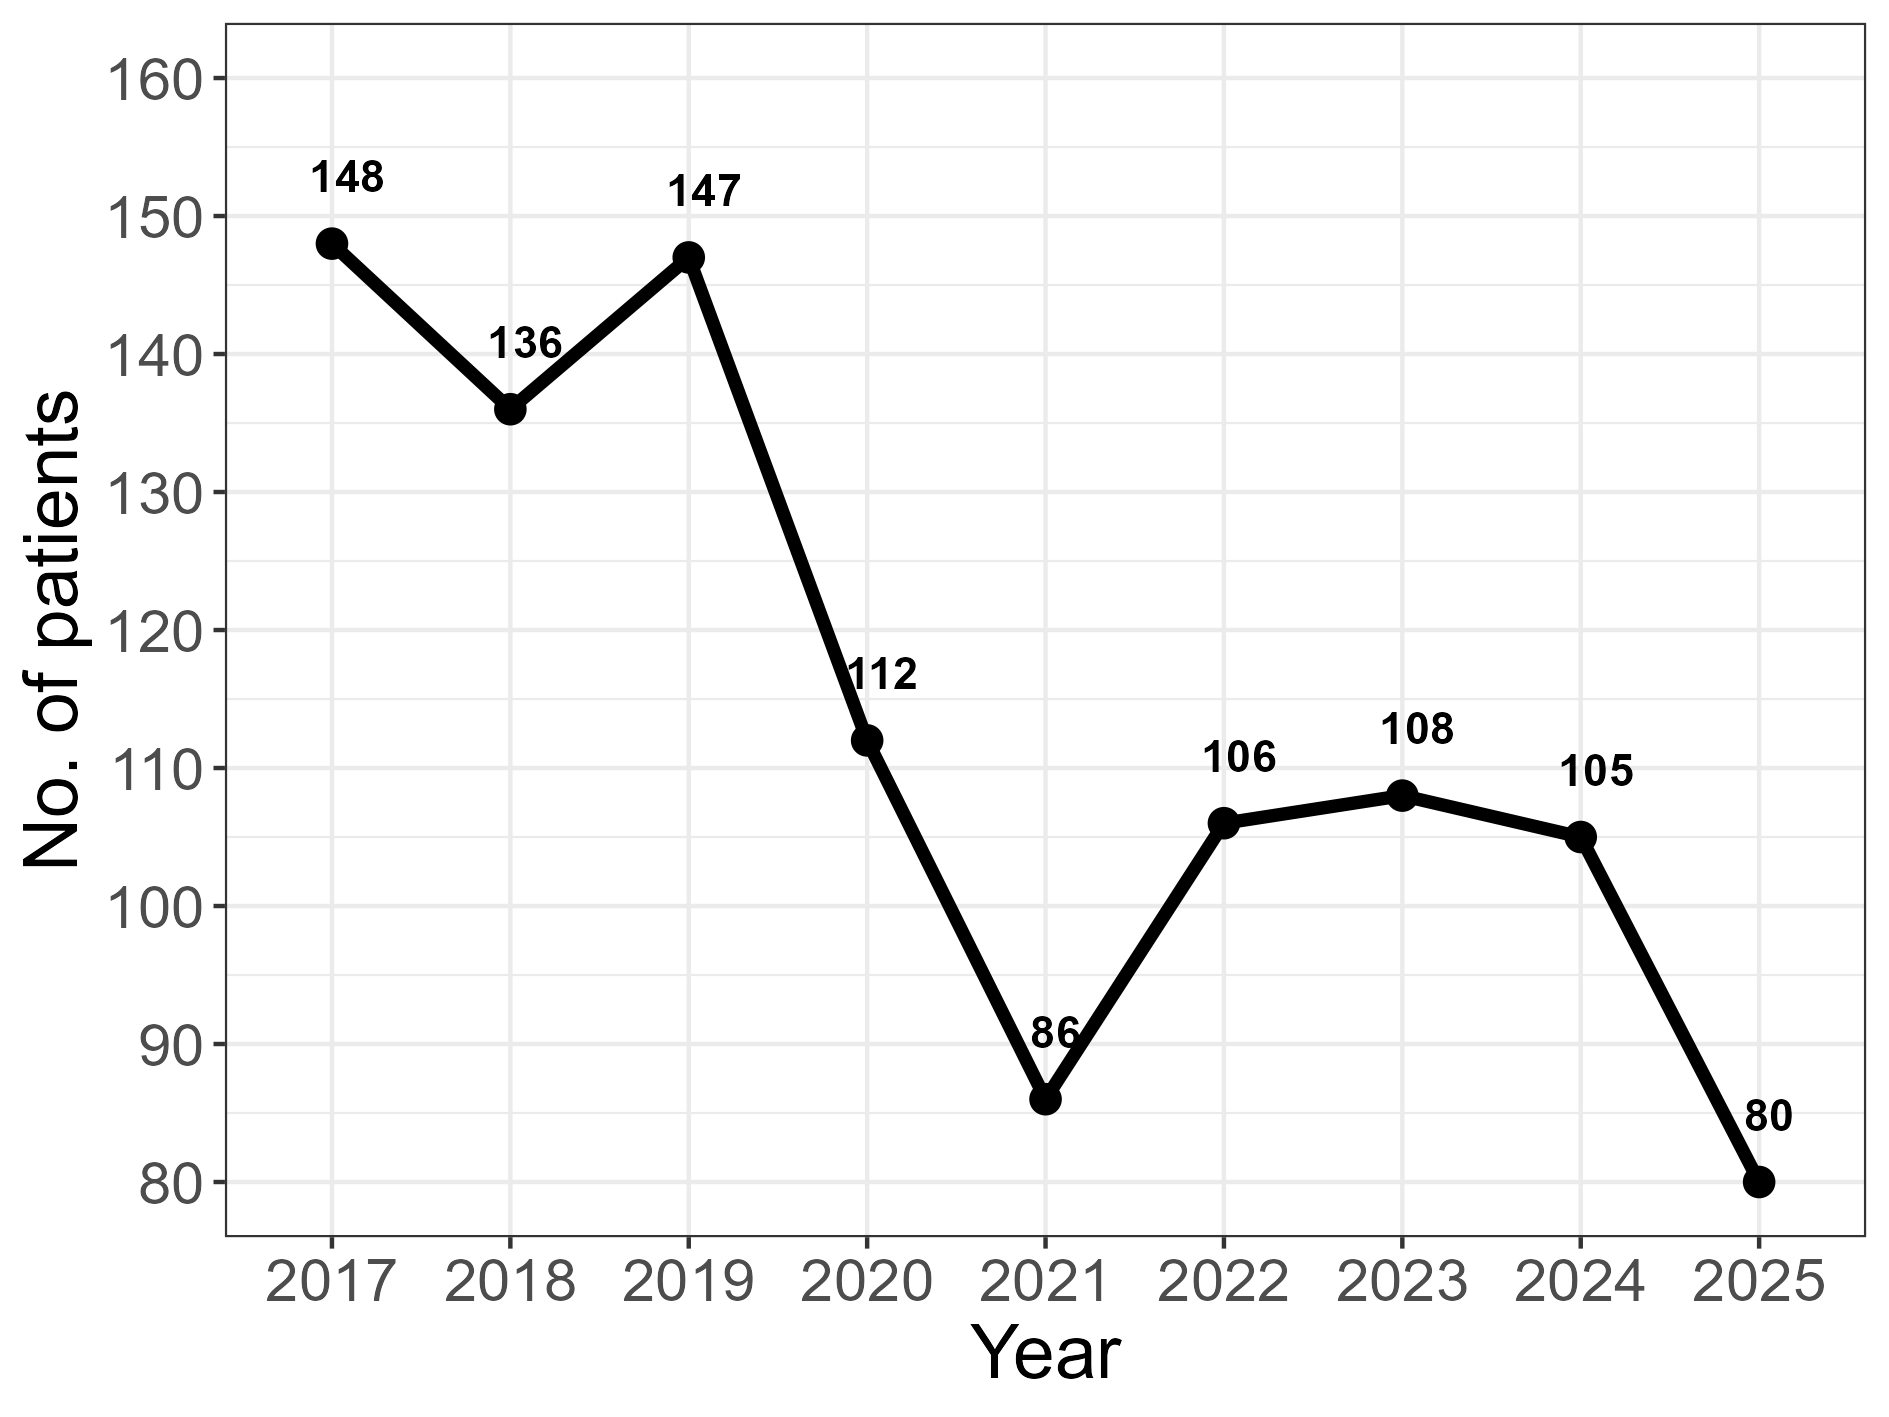
\includegraphics[width=0.75\textwidth]{nutri_paren_id_tend.png}
    \caption{Number of unique patients aged 0--17 years identified as probable CIF cases (parenteral nutrition $\geq$ 60 daily units) per year, Brazil, 2017--2025.}
    \label{fig:fic_por_ano}
\end{figure}

The trajectory of prevalence estimates warrants careful interpretation. The sharp decline observed during 2020 and 2021 is unlikely to reflect a true reduction in the underlying incidence of CIF, a condition whose aetiology is predominantly congenital and therefore not plausibly affected by a pandemic in the short term. A more likely explanation is that the collapse in non-urgent hospital capacity during the COVID-19 crisis restricted access to the prolonged parenteral nutrition required for CIF management, effectively rendering a portion of the affected population invisible to administrative records. This interpretation is further supported by the fact that the post-pandemic recovery in case counts, while real, remained below pre-pandemic levels. Consistent with the hypothesis that some patients who were unable to access treatment during 2020 and 2021 may not have survived to be counted in subsequent years. Taken together, these observations suggest that the prevalence estimates reported here, including the pre-pandemic figures, are likely to represent a lower bound of the true burden of paediatric CIF in Brazil, reflecting not the full extent of the condition but rather the subset of cases that successfully accessed prolonged hospital-based parenteral nutrition within the SUS. The extent to which this underestimation is driven by access barriers, rather than by true scarcity of cases, is further examined in the final section of these results.

\subsection*{Clinical and Demographic Profile of Identified CIF Cases}

The clinical and demographic characterisation of the 971 patients identified through the PN-based strategy reveals several features that are consistent with the international literature on paediatric CIF and that illuminate important aspects of how this population is managed within the Brazilian health system.

\subsubsection*{Age and Sex}

The mean age of patients at admission was markedly low, remaining below 1.5 years throughout the study period and falling as low as 0.81 years in 2022, indicating a strong concentration of cases in the first months of life (Figure~\ref{fig:idade}). This is consistent with the known epidemiology of the condition, in which Short Bowel Syndrome most commonly results from neonatal surgical complications such as necrotising enterocolitis, intestinal atresia, or midgut volvulus, conditions that manifest at or shortly after birth \cite{wales2004neonatal, squires2012natural}. Males accounted for 53.6\% of the sample overall (Figure~\ref{fig:sexo}), a slight male predominance that contrasts with findings from some international studies suggesting a higher prevalence of SBS-related CIF in females \cite{massironi2020understanding}, though the difference observed here is modest.

\begin{figure}[H]
    \centering
    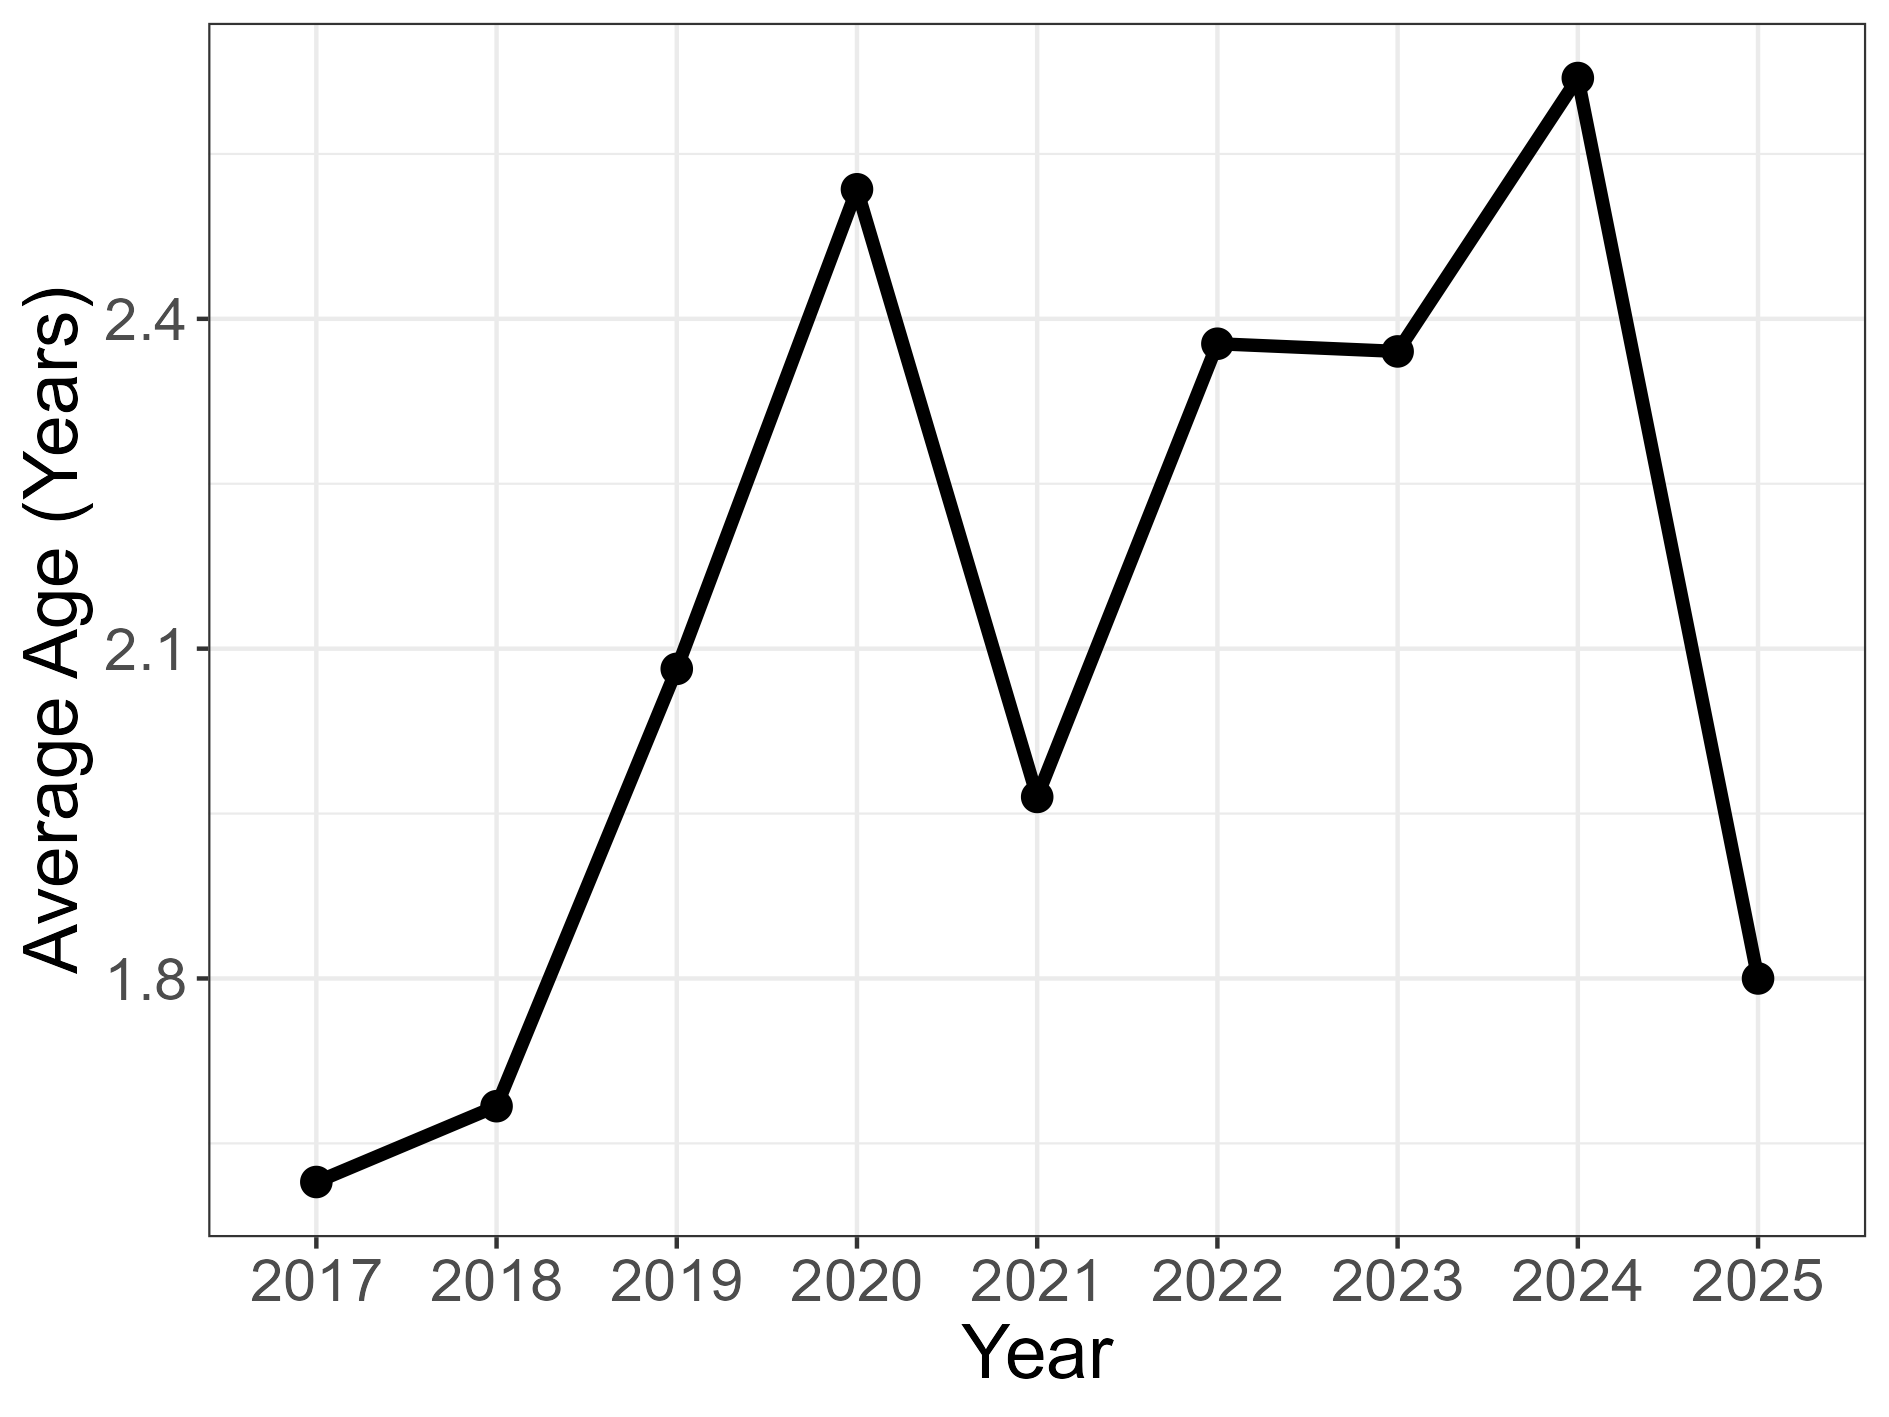
\includegraphics[width=0.75\textwidth]{nutri_paren_id_idade.png}
    \caption{Mean age (in years) of identified CIF patients at time of admission, by year, Brazil, 2017--2025.}
    \label{fig:idade}
\end{figure}

\begin{figure}[H]
    \centering
    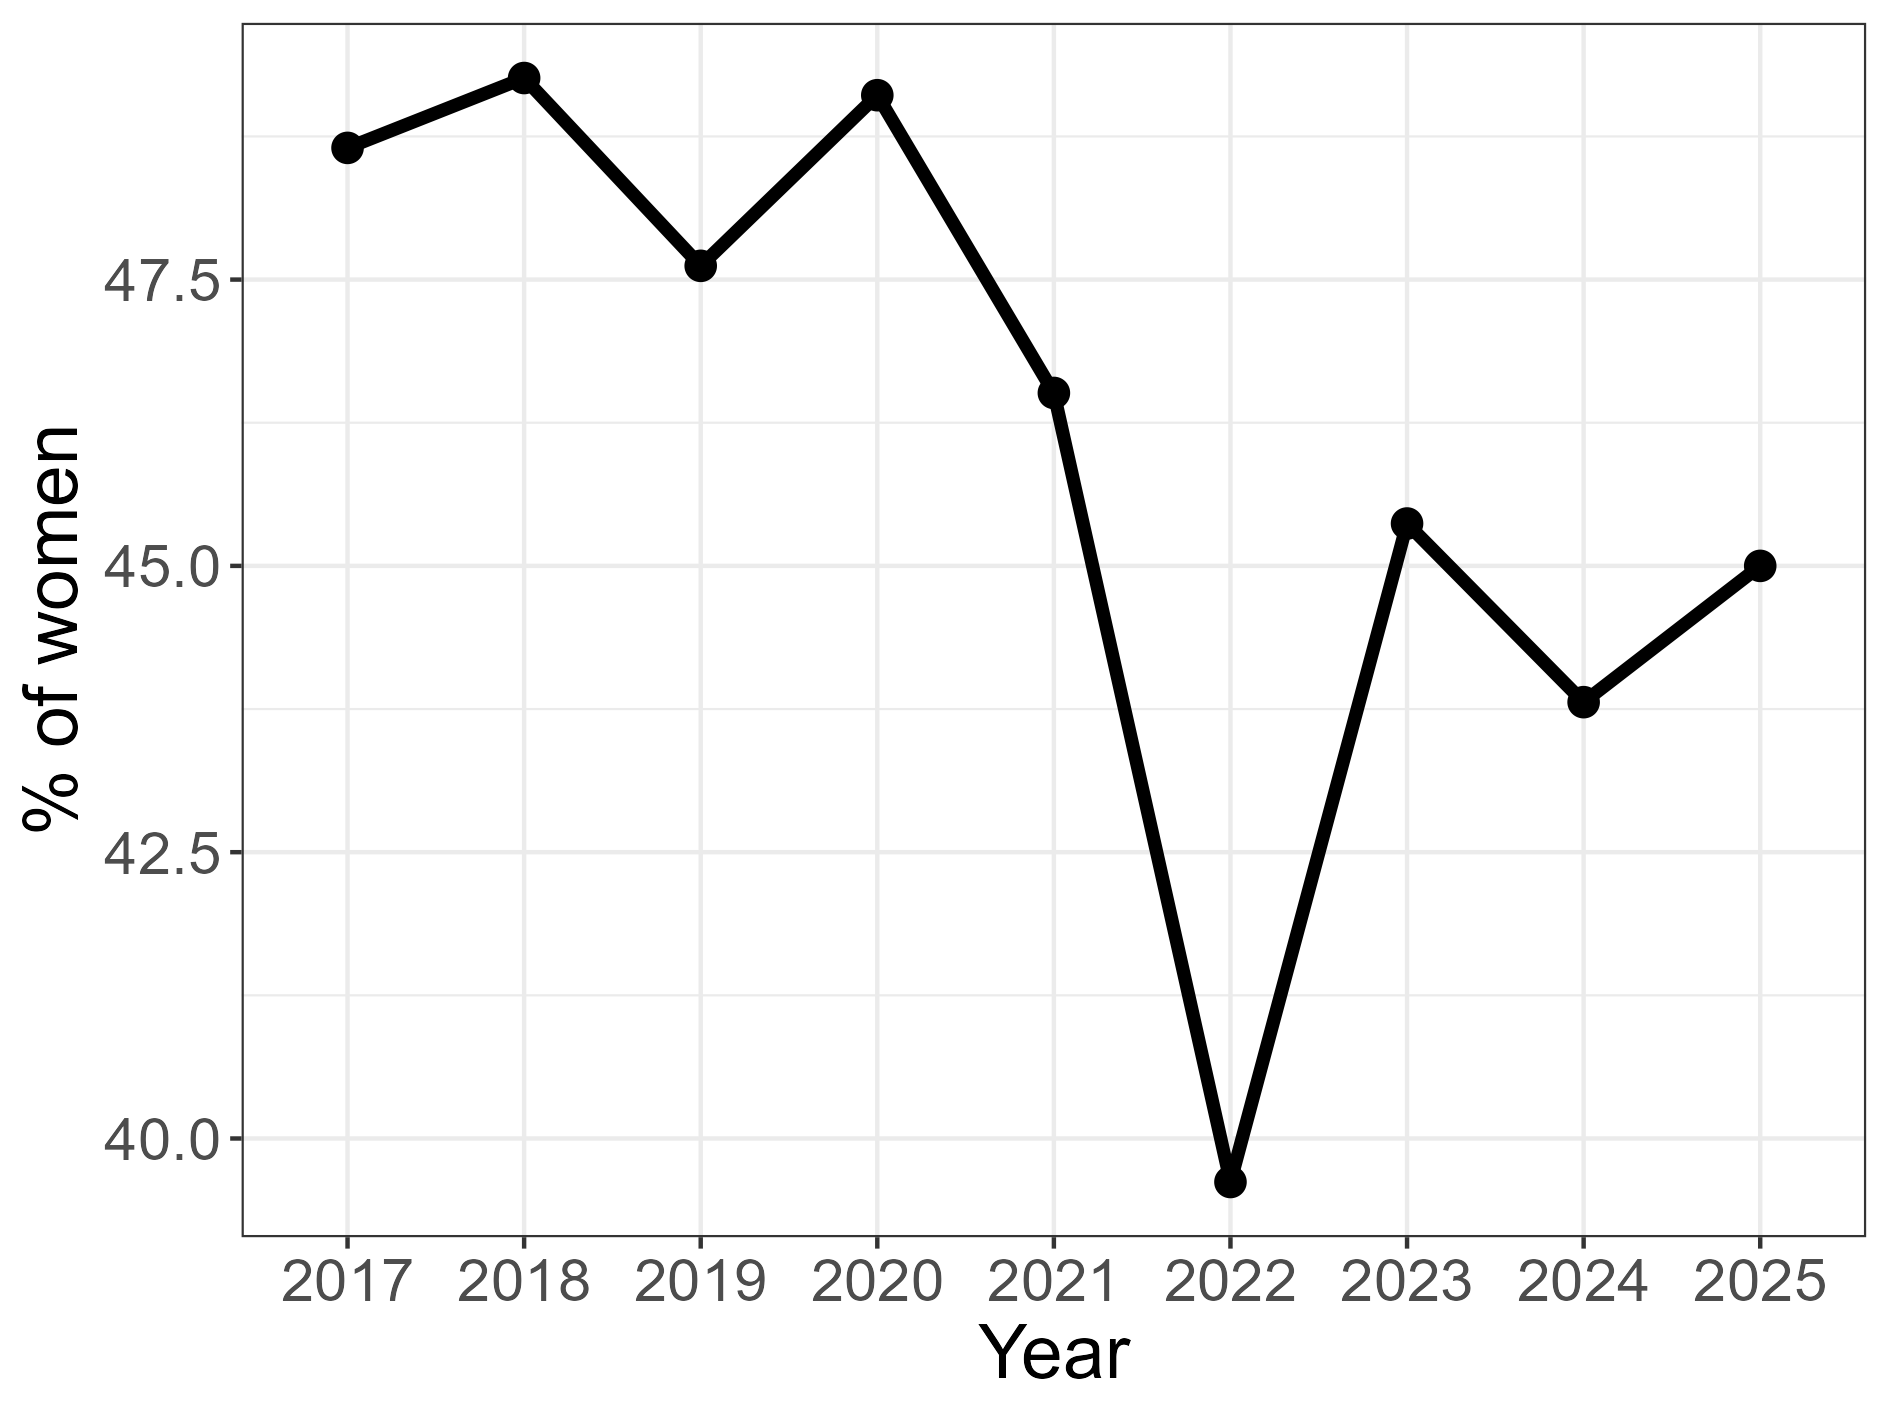
\includegraphics[width=0.75\textwidth]{nutri_paren_id_sexo.png}
    \caption{Proportion of female patients among identified CIF cases, by year, Brazil, 2017--2025.}
    \label{fig:sexo}
\end{figure}

\subsubsection*{Race and Ethnicity}

The proportion of white patients in the CIF cohort exceeded their share in the general Brazilian population throughout most of the study period, ranging from approximately 42\% to 52\% (Figure~\ref{fig:raca}). While this finding should be interpreted cautiously given the known underreporting of race/ethnicity in SIH-SUS records, it is nonetheless suggestive of differential access to prolonged hospital-based parenteral nutrition across racial groups. A pattern that, represent a significant equity concern in the management of a condition whose outcomes are strongly dependent on the timely and sustained availability of this treatment.

\begin{figure}[H]
    \centering
    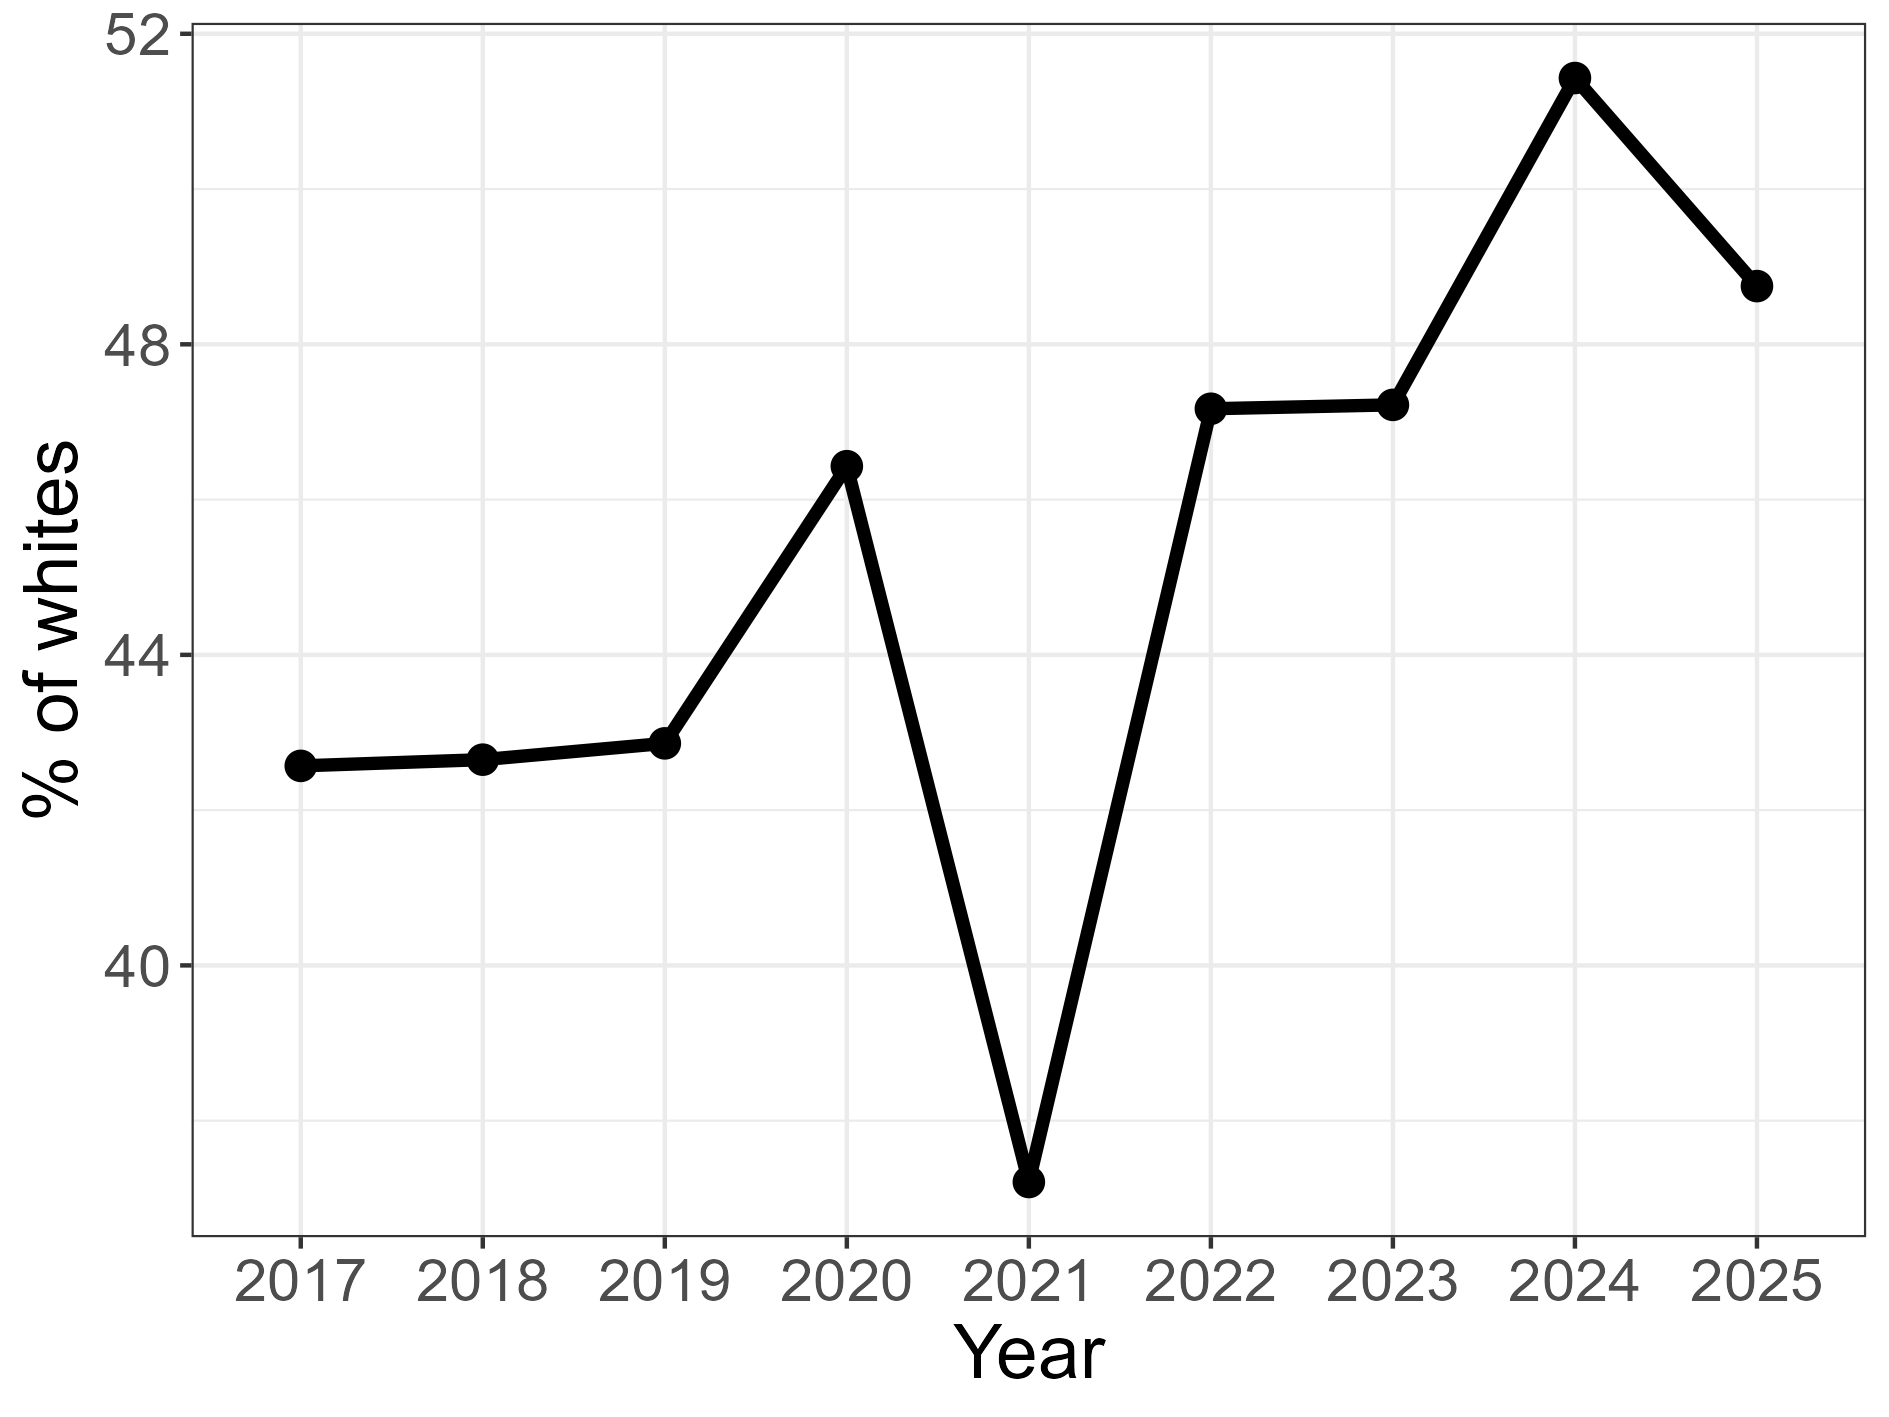
\includegraphics[width=0.75\textwidth]{nutri_paren_id_raca_cor.png}
    \caption{Proportion of white patients among identified CIF cases, by year, Brazil, 2017--2025.}
    \label{fig:raca}
\end{figure}

\subsubsection*{Clinical Profile: Diagnoses and Procedures}

The primary diagnoses and co-registered procedures recorded for patients with PN lasting 60 or more days reveal a strong association between CIF and neonatal morbidity in Brazil. The five most frequent primary diagnoses were other preterm newborns (16.0\%), unspecified respiratory distress of the newborn (10.3\%), respiratory distress syndrome of the newborn (10.0\%), other respiratory distress of the newborn (4.6\%), and extreme immaturity (3.8\%) (Table~\ref{tab:diagnosticos}). Similarly, the most commonly co-registered procedures were treatment of respiratory and cardiovascular disorders specific to the neonatal period (33.65\% of cases), treatment of disorders related to gestational duration and fetal growth (20.2\%), treatment of other bacterial diseases (7.6\%), treatment involving multiple surgeries (4.7\%), and treatment of other disorders originating in the perinatal period (4.2\%) (Table~\ref{tab:procedimentos}). Taken together, these findings indicate that, in the Brazilian context, paediatric CIF is predominantly encountered as a complication of premature birth and its associated neonatal morbidities, rather than being primarily attributable to congenital enteropathies or motility disorders, conditions that are more prominently represented in European cohorts \cite{beath2011trends, antunes2020portuguese}. This may reflect, at least in part, the epidemiological profile of neonatal care in Brazil, where prematurity rates remain high and access to specialised neonatal intensive care is unequally distributed across regions.

\begin{table}[ht]
\centering
\caption{Five most frequent primary ICD-10 diagnoses among identified CIF patients (parenteral nutrition $\geq$ 60 daily units), aged 0--17 years, Brazil, 2017--2025.}
\label{tab:diagnosticos}
\renewcommand{\arraystretch}{1.3}
\begin{tabular}{lc}
\toprule
Diagnosis & \% of cases \\
\midrule
Other preterm newborns & 16.0\% \\
Unspecified respiratory distress of the newborn & 10.3\% \\
Respiratory distress syndrome of the newborn & 10.0\% \\
Other respiratory distress of the newborn & 4.6\% \\
Extreme immaturity & 3.8\% \\
\bottomrule
\end{tabular}
\end{table}

\begin{table}[ht]
\centering
\caption{Five most frequent co-registered procedures among identified CIF patients (parenteral nutrition $\geq$ 60 daily units), aged 0--17 years, Brazil, 2017--2025.}
\label{tab:procedimentos}
\renewcommand{\arraystretch}{1.3}
\begin{tabular}{lc}
\toprule
Procedure & \% of cases \\
\midrule
Treatment of respiratory and cardiovascular disorders specific to the neonatal & 33.65\% \\
Treatment of disorders related to gestational duration and fetal growth & 20.2\% \\
Treatment of other bacterial diseases & 7.6\% \\
Treatment involving multiple surgeries & 4.7\% \\
Treatment of other disorders originating in the perinatal period & 4.2\% \\
\bottomrule
\end{tabular}
\end{table}

\subsubsection*{Healthcare Utilisation}

Patients identified as CIF cases exhibited an intensive pattern of healthcare use. The mean number of hospital admissions per patient ranged from 2.5 in 2017 to 4.5 in 2024, with an overall trend toward increasing fragmentation of care over the study period (Figure~\ref{fig:internacoes}). The mean duration of individual admissions remained close to 60 daily units throughout, consistent with the minimum threshold used to define CIF in this study (Figure~\ref{fig:duracao}). However, when the total number of daily units is accumulated across all admissions per patient, the aggregate hospitalisation burden is substantially higher, with mean cumulative daily units reaching approximately 150--165 per year in the more recent part of the study period (Figure~\ref{fig:diarias}). This pattern of multiple sequential admissions of moderate individual duration, rather than single prolonged hospitalisations, may reflect operational constraints of the SUS reimbursement system, including the possibility that administrative limits on admission duration incentivise premature discharge and subsequent readmission, rather than a genuine clinical resolution between hospitalisations.

\begin{figure}[H]
    \centering
    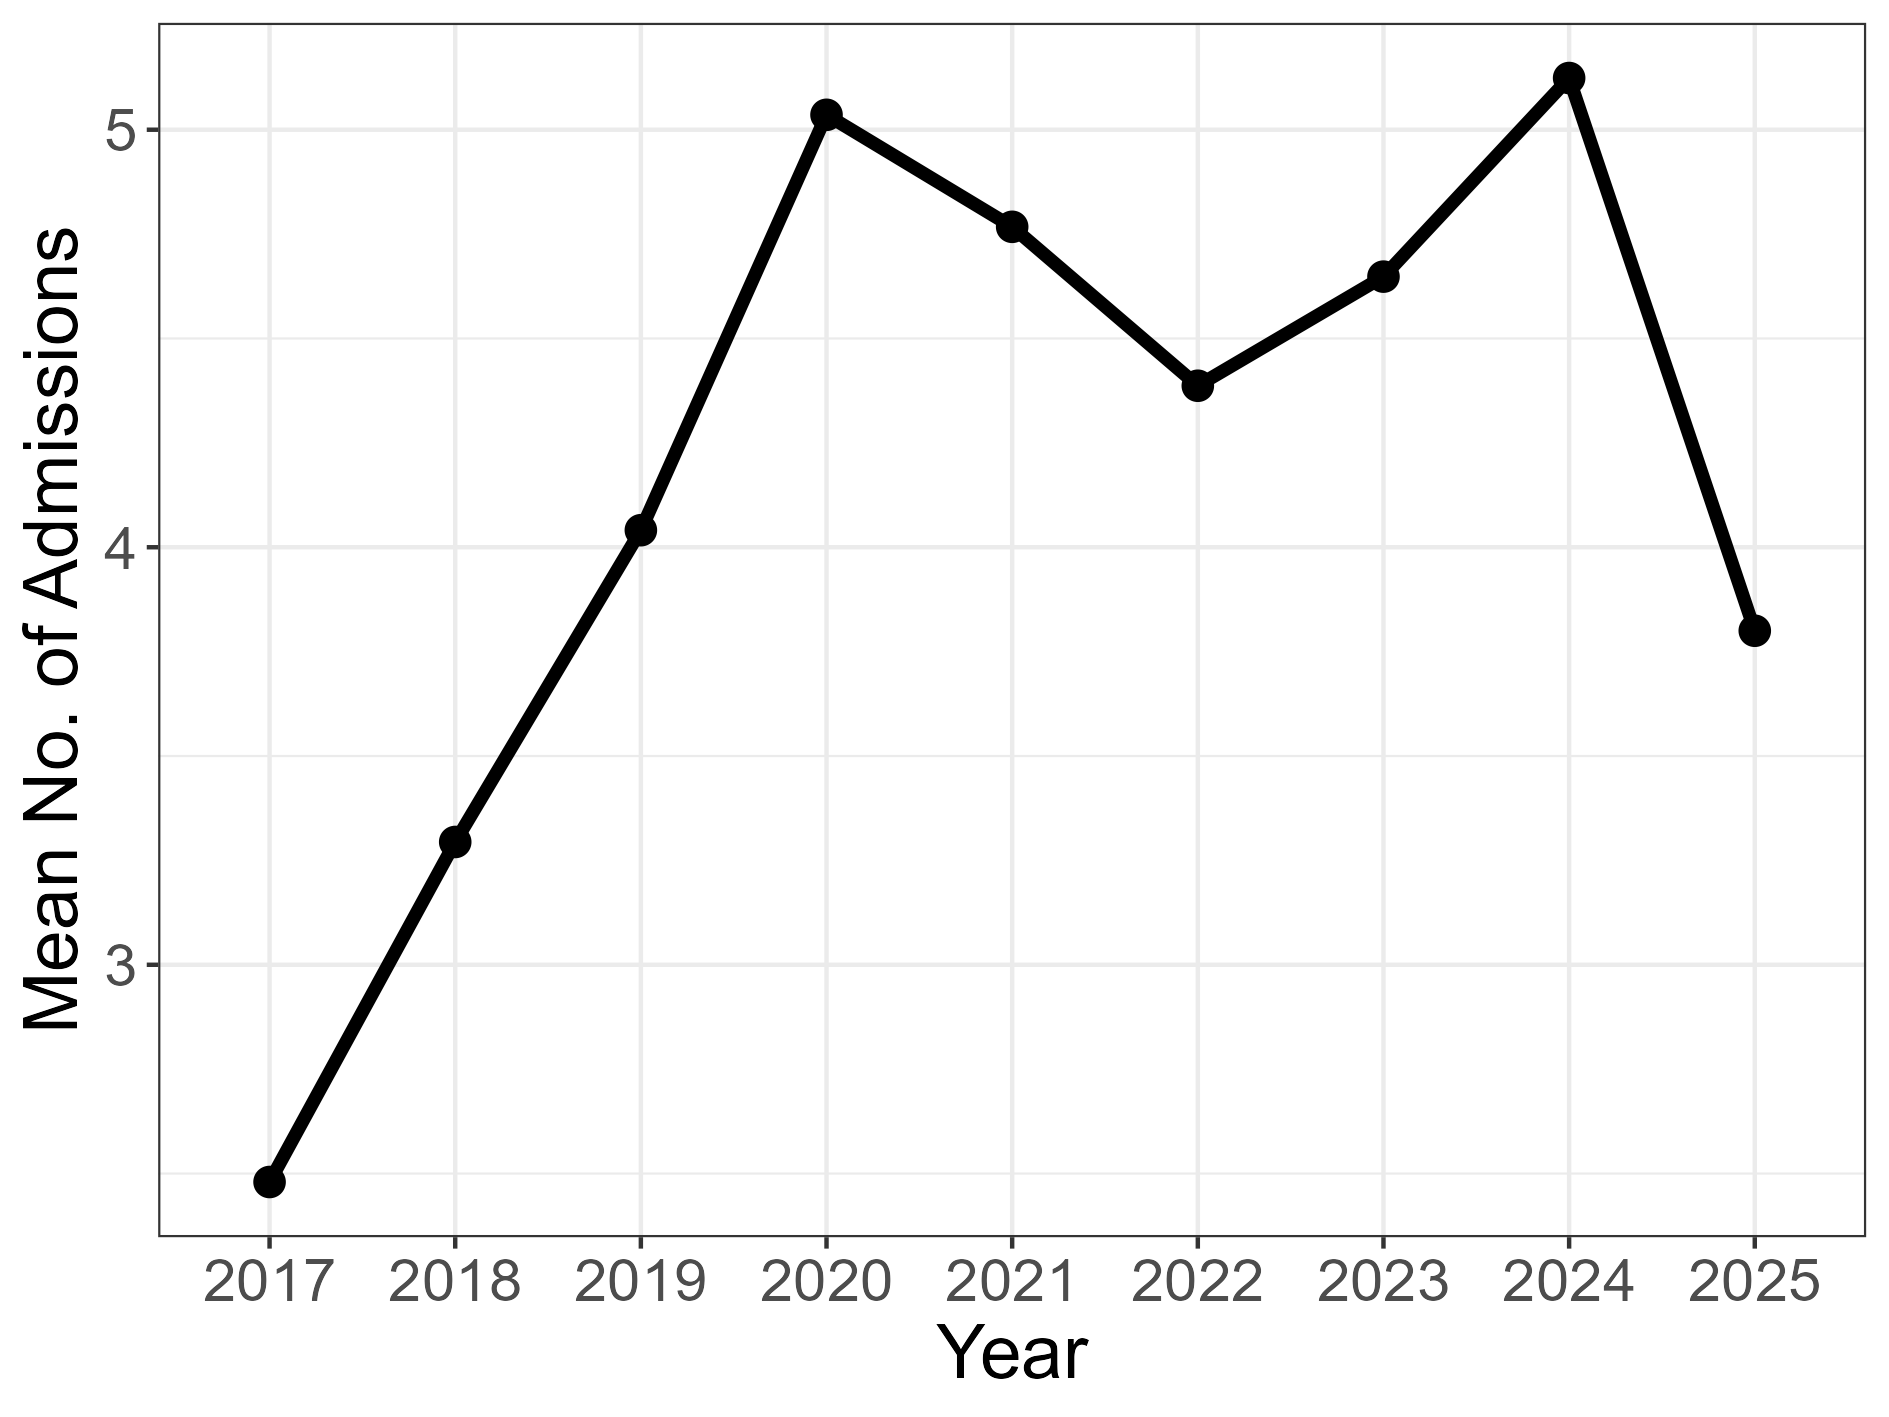
\includegraphics[width=0.75\textwidth]{nutri_paren_id_total_internacoes.png}
    \caption{Mean number of hospital admissions per identified CIF patient, by year, Brazil, 2017--2025.}
    \label{fig:internacoes}
\end{figure}

\begin{figure}[H]
    \centering
    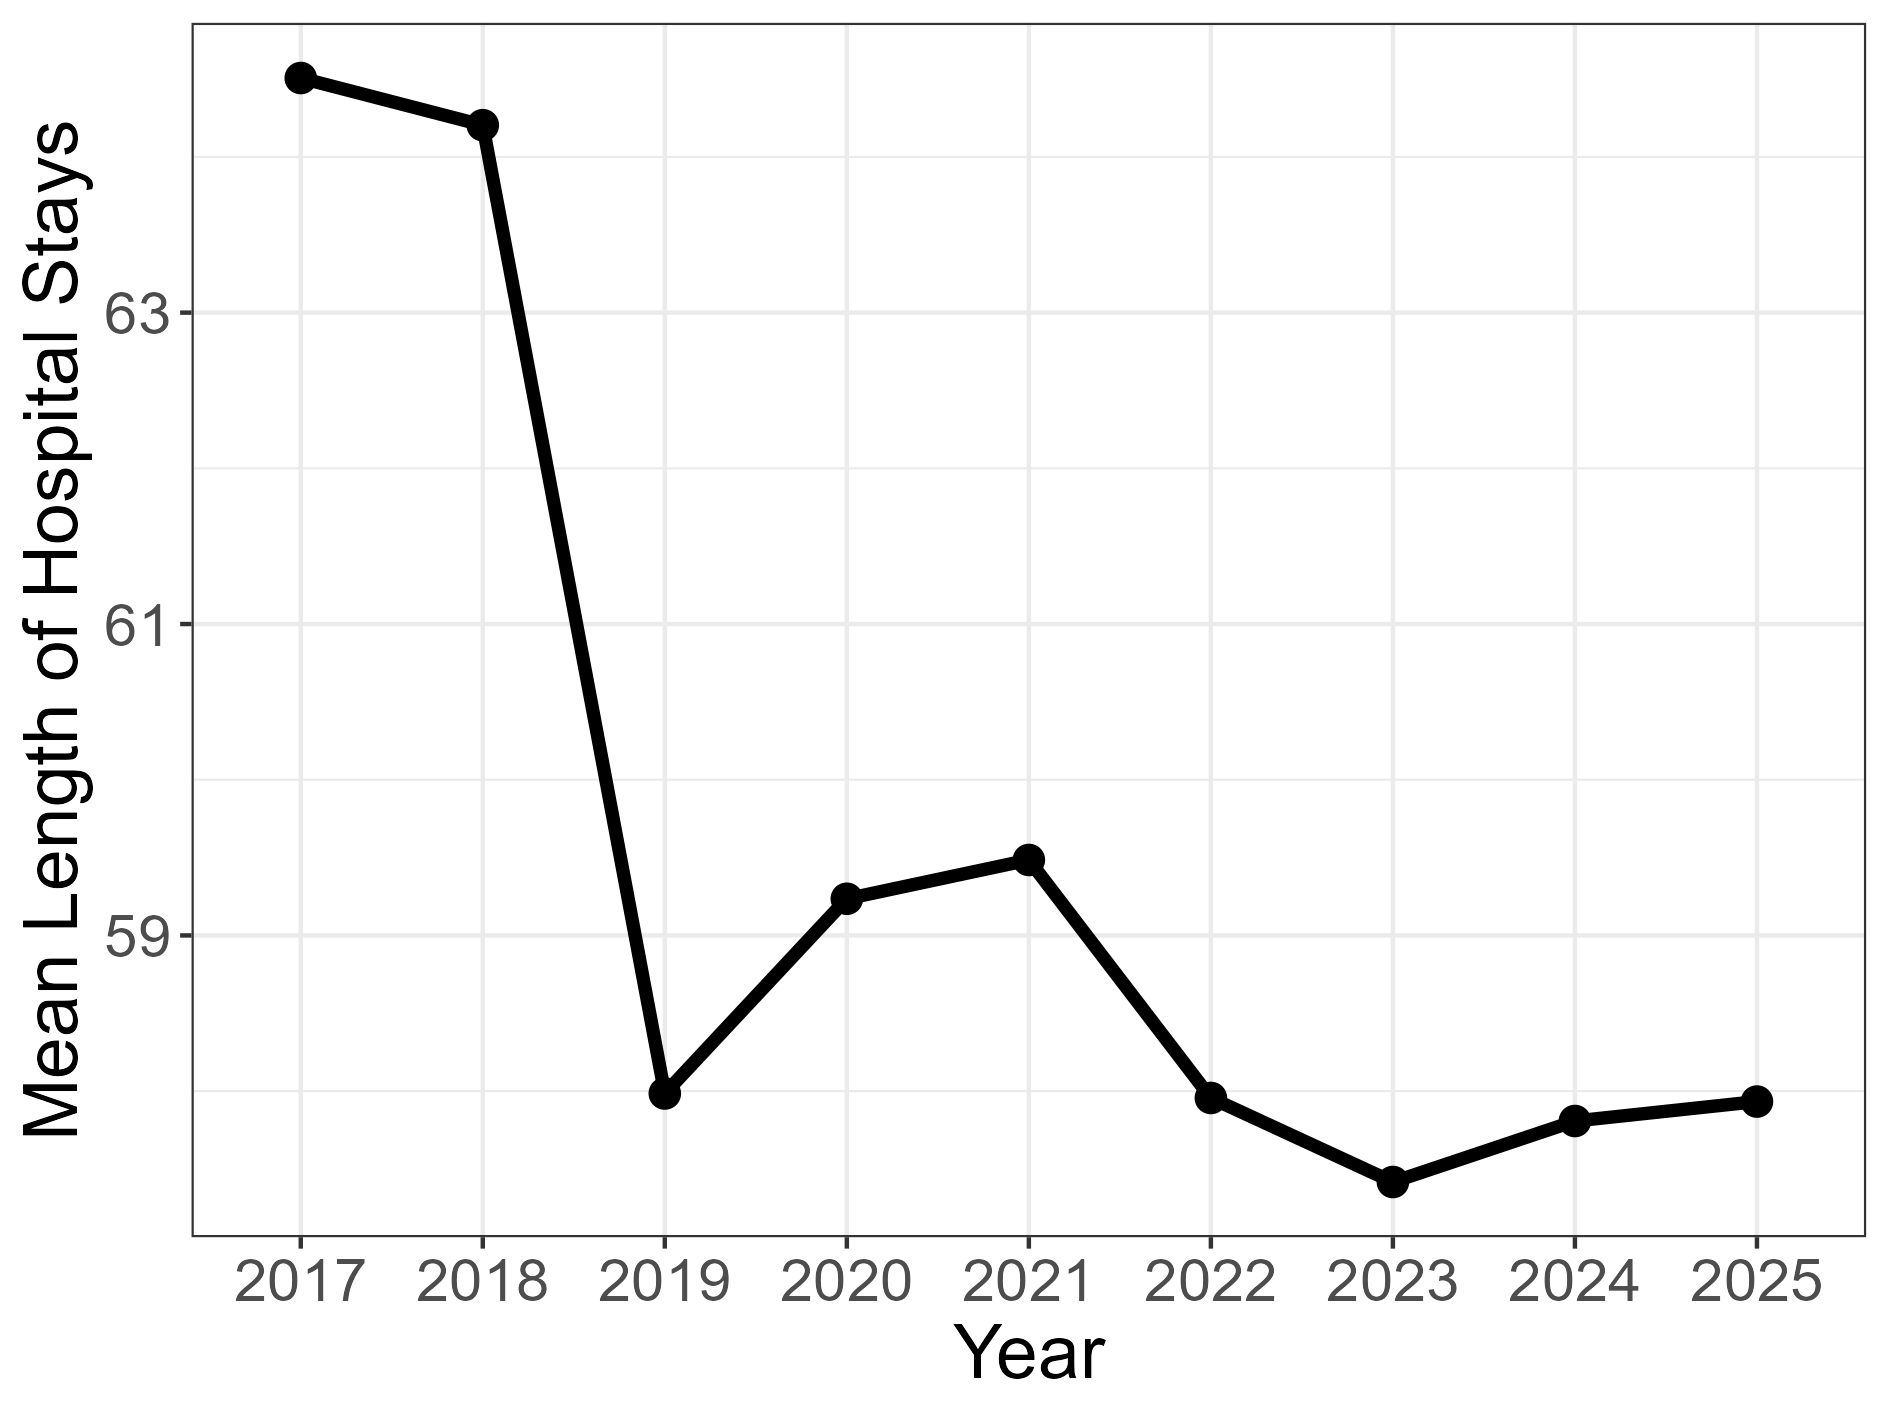
\includegraphics[width=0.75\textwidth]{nutri_paren_id_duracao_internacoes.png}
    \caption{Mean duration of individual hospital admissions (daily units) among identified CIF patients, by year, Brazil, 2017--2025.}
    \label{fig:duracao}
\end{figure}

\begin{figure}[H]
    \centering
    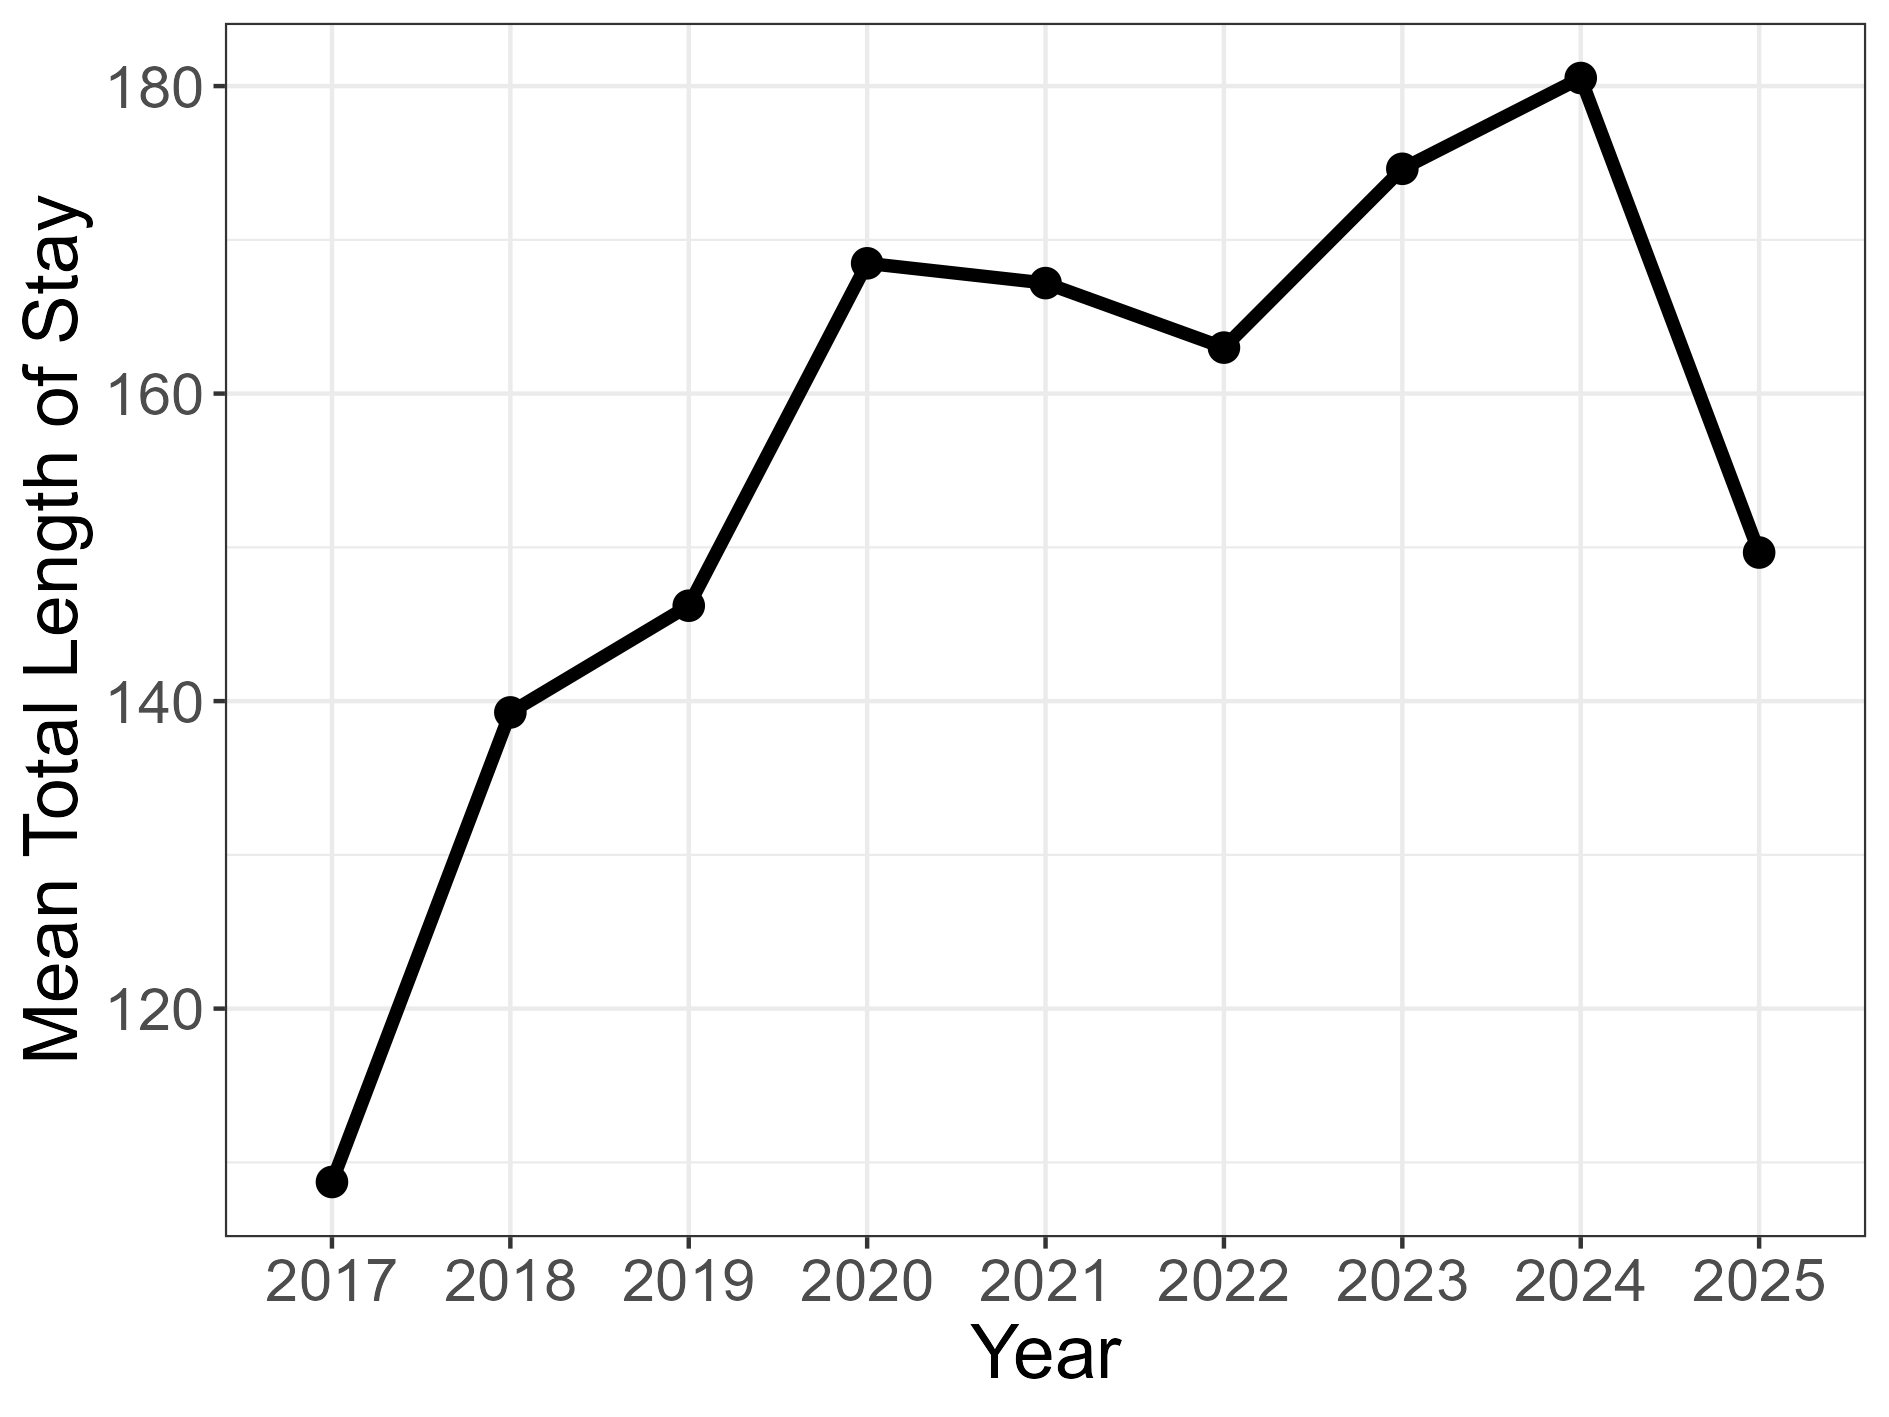
\includegraphics[width=0.75\textwidth]{nutri_paren_id_total_diarias.png}
    \caption{Mean cumulative daily units of parenteral nutrition per identified CIF patient, by year, Brazil, 2017--2025.}
    \label{fig:diarias}
\end{figure}

The in-hospital mortality rate among CIF patients fluctuated between approximately 9\% and 15\% across the study years (Figure~\ref{fig:obito}). While this rate is lower than the mortality burden that would be expected in the complete absence of treatment, it remains substantially higher than what is observed in well-resourced CIF programmes in high-income countries, where survival rates of 85\% or more have been reported with adequate parenteral nutrition \cite{mukhopadhyay2019}. The proportion of patients discharged with clinical improvement exceeded 50\% in several years, reaching as high as 58\% in 2018 (Figure~\ref{fig:alta}), but showed a declining trend in the most recent years of the study period, which warrants monitoring.

\begin{figure}[H]
    \centering
    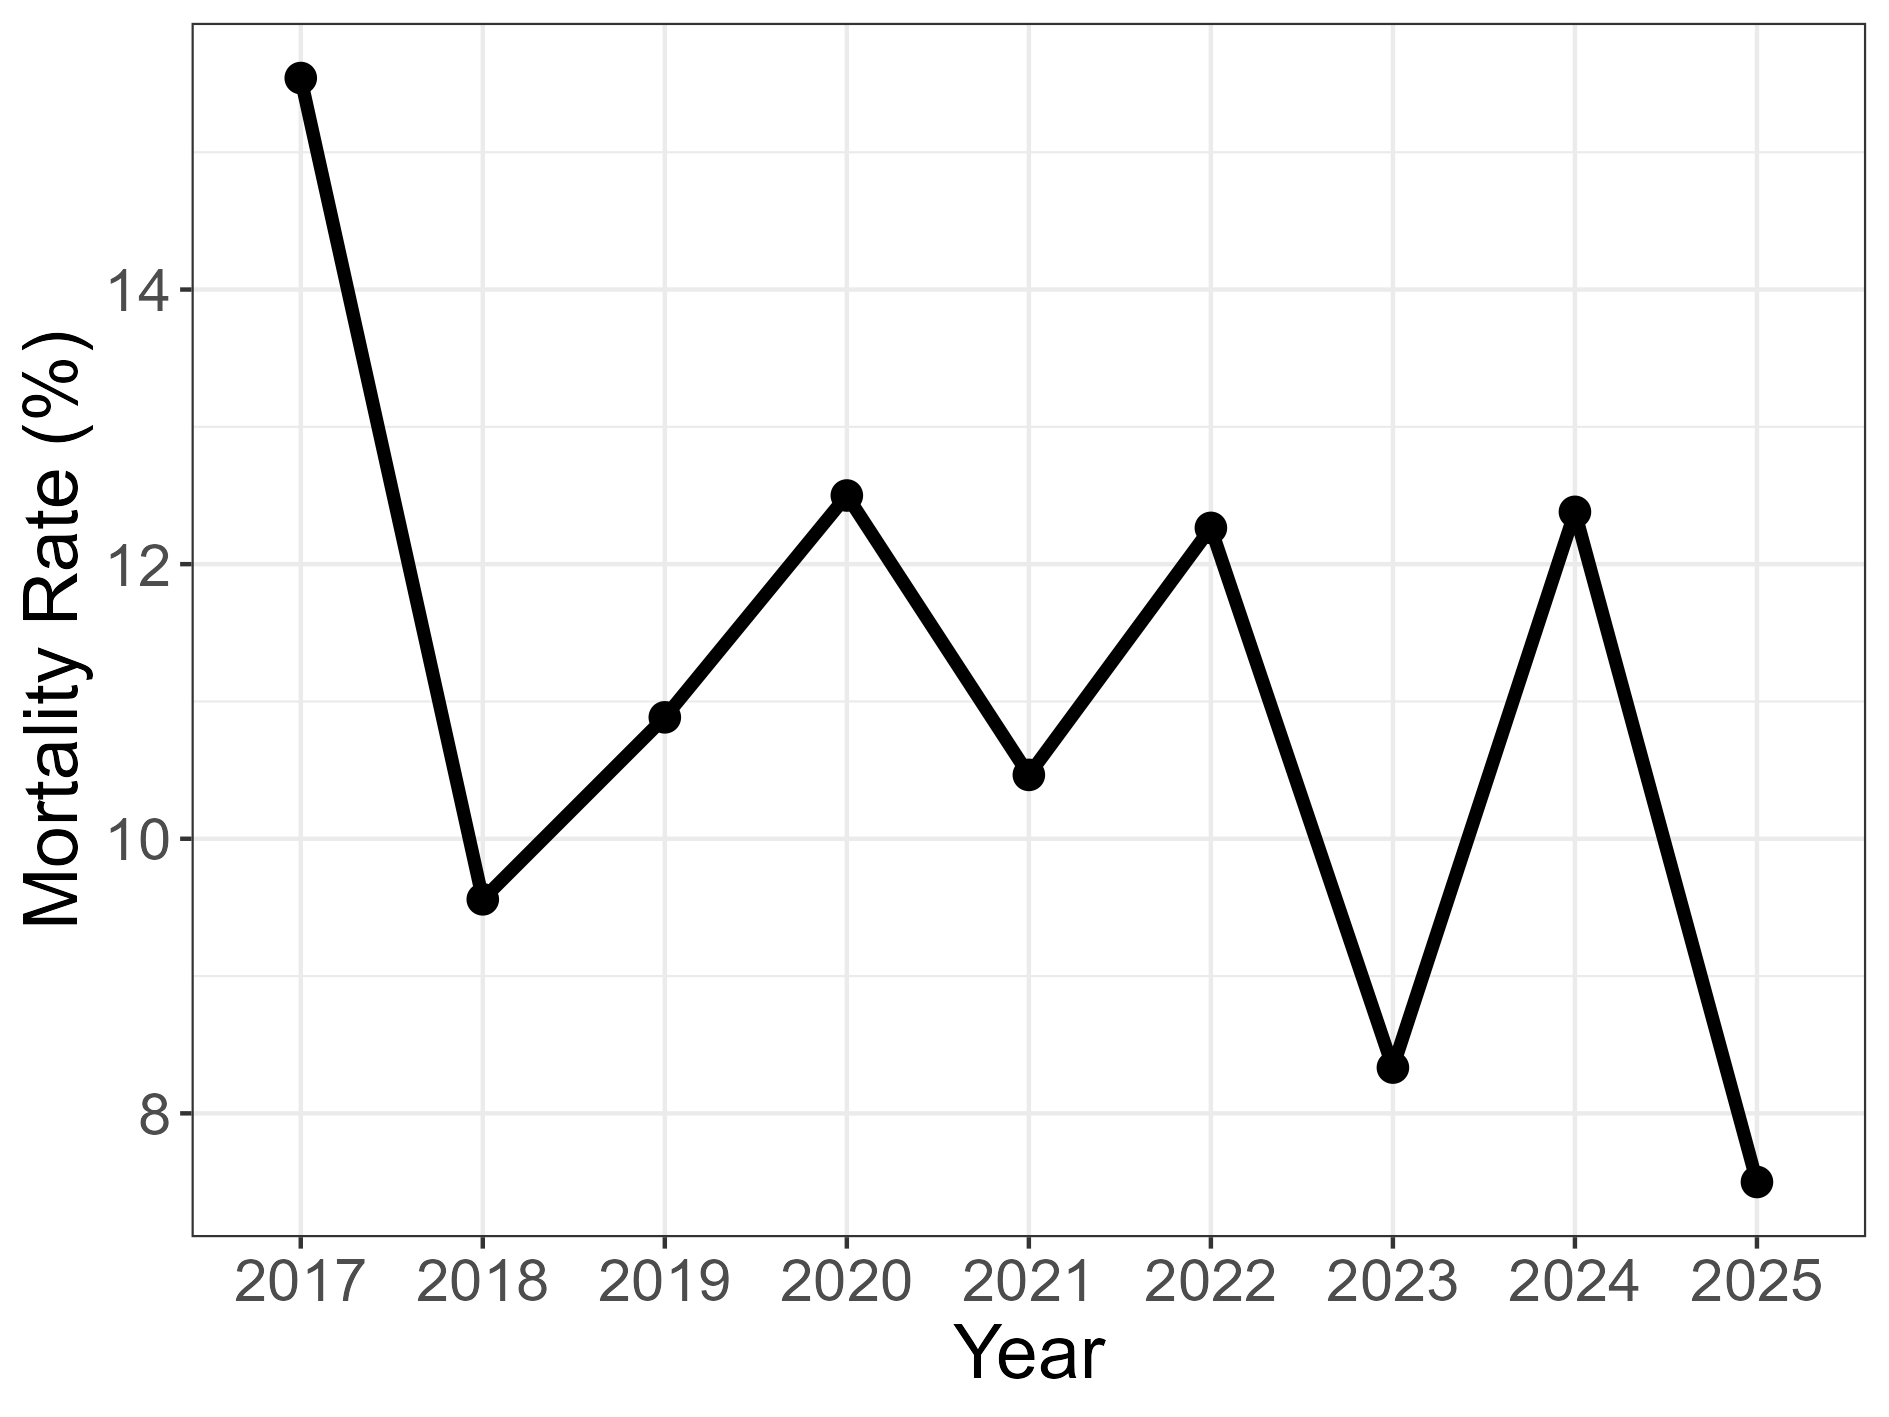
\includegraphics[width=0.75\textwidth]{nutri_paren_id_obito.png}
    \caption{In-hospital mortality rate among identified CIF patients, by year, Brazil, 2017--2025.}
    \label{fig:obito}
\end{figure}

\begin{figure}[H]
    \centering
    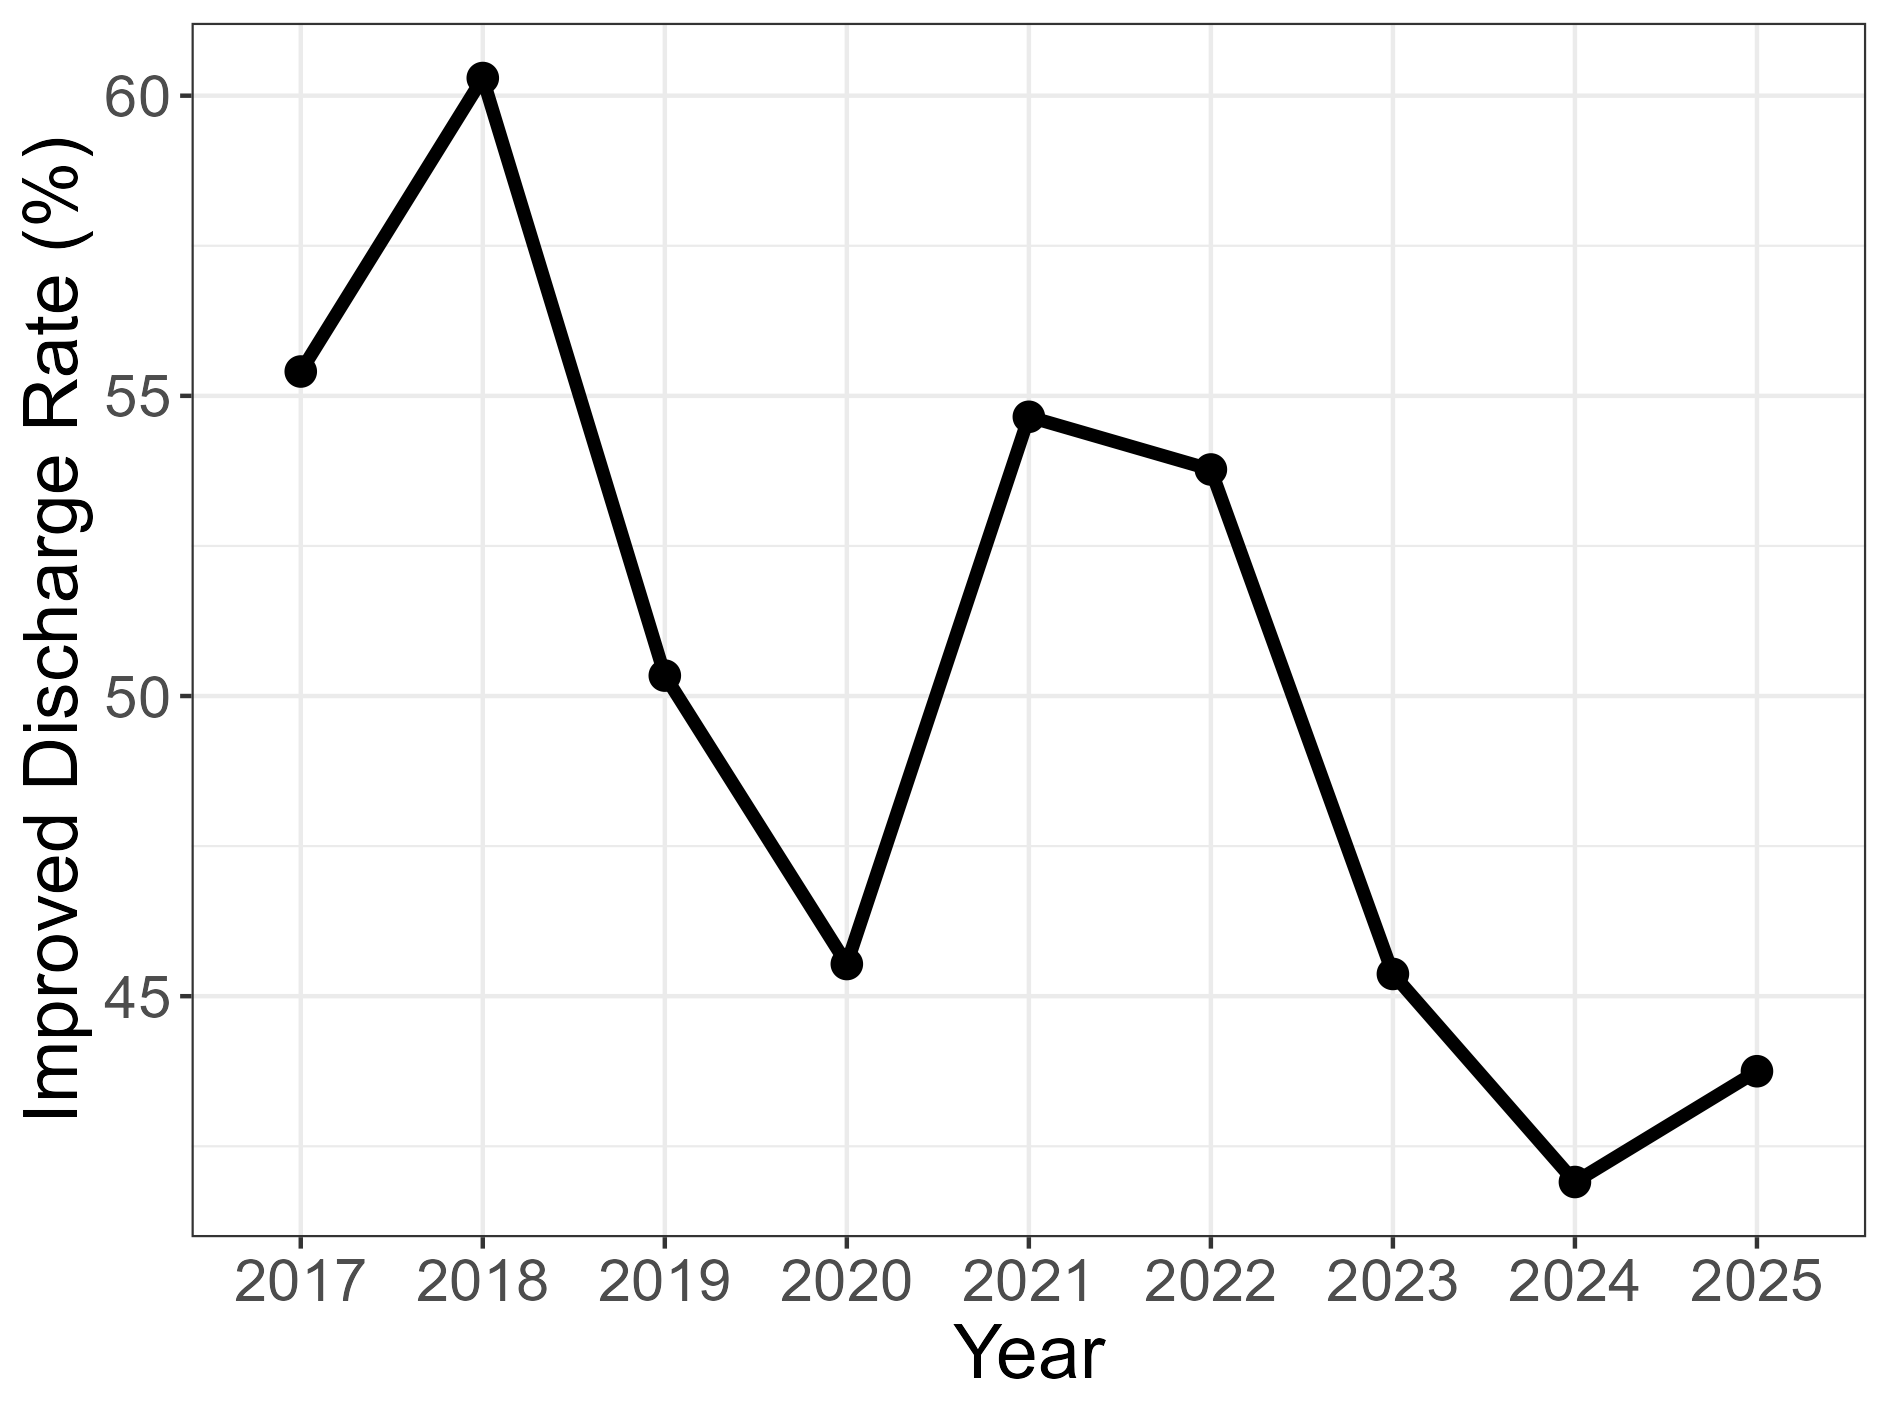
\includegraphics[width=0.75\textwidth]{nutri_paren_id_alta_melhorada.png}
    \caption{Proportion of identified CIF patients discharged with clinical improvement (\textit{alta melhorada}), by year, Brazil, 2017--2025.}
    \label{fig:alta}
\end{figure}

\subsubsection*{Geographic Distribution and Access to Care}

The geographic distribution of CIF cases and treating hospitals reveals a pronounced mismatch between the location of patients and the location of specialised care. Throughout the study period, the hospitals providing prolonged parenteral nutrition to paediatric patients were concentrated in a small number of municipalities, predominantly in the South and Southeast regions of Brazil, while patients resided in a considerably wider set of localities (Figure~\ref{fig:mapa}). More than half of all identified CIF patients (consistently above 50\% in most years of the study period) were required to travel outside their municipality of residence to access treatment (Figure~\ref{fig:deslocamento}), with a mean travel distance of approximately 70 kilometres between the patient's residential postal code centroid and the treating hospital's municipality (Figure~\ref{fig:distancia}). This level of geographic displacement, imposed on families of infants and young children requiring continuous and life-sustaining nutritional support, constitutes a significant access barrier and is consistent with the broader pattern of geographic concentration of specialised paediatric care in Brazil. The near-total absence of identified CIF cases in the North, Northeast and Central-West regions of the country further suggests that the burden of unmet need for CIF treatment may be disproportionately concentrated in the regions with the lowest healthcare infrastructure density.

\begin{figure}[H]
    \centering
    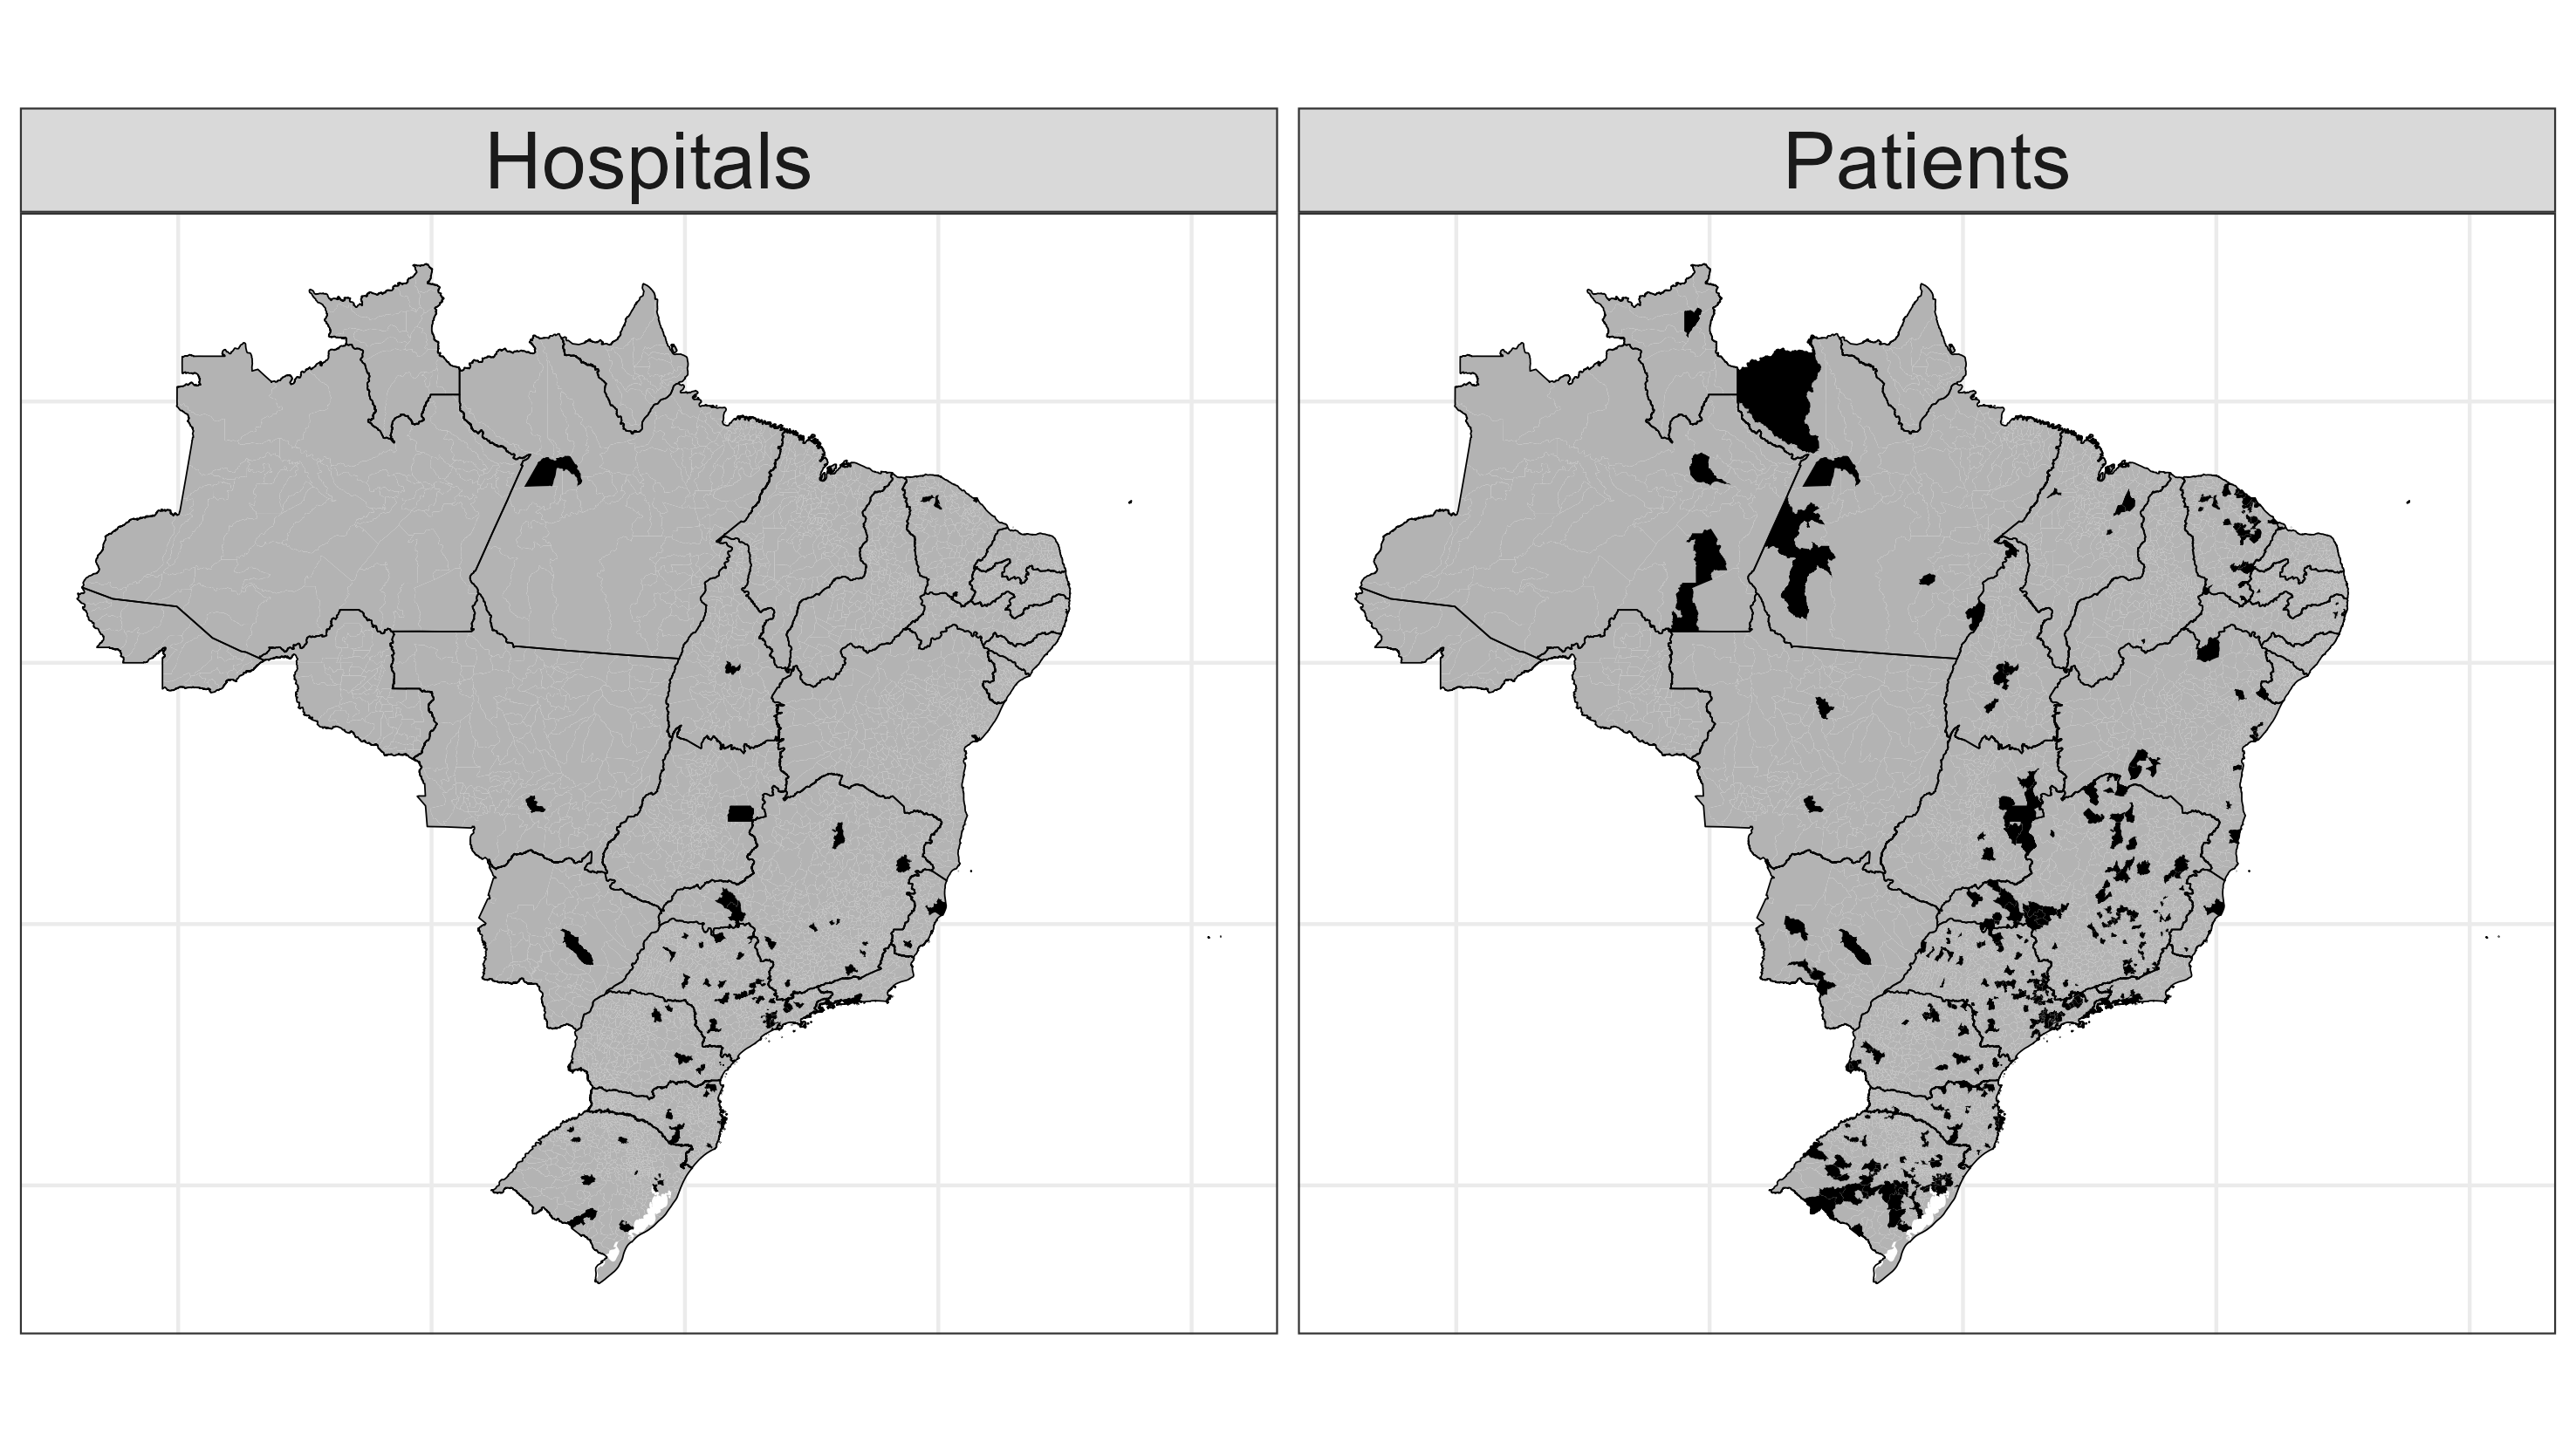
\includegraphics[width=0.90\textwidth]{nutri_paren_id_mapa.png}
    \caption{Geographic distribution of hospitals providing parenteral nutrition (left) and municipalities of residence of identified CIF patients (right), Brazil, 2017--2024.}
    \label{fig:mapa}
\end{figure}

\begin{figure}[H]
    \centering
    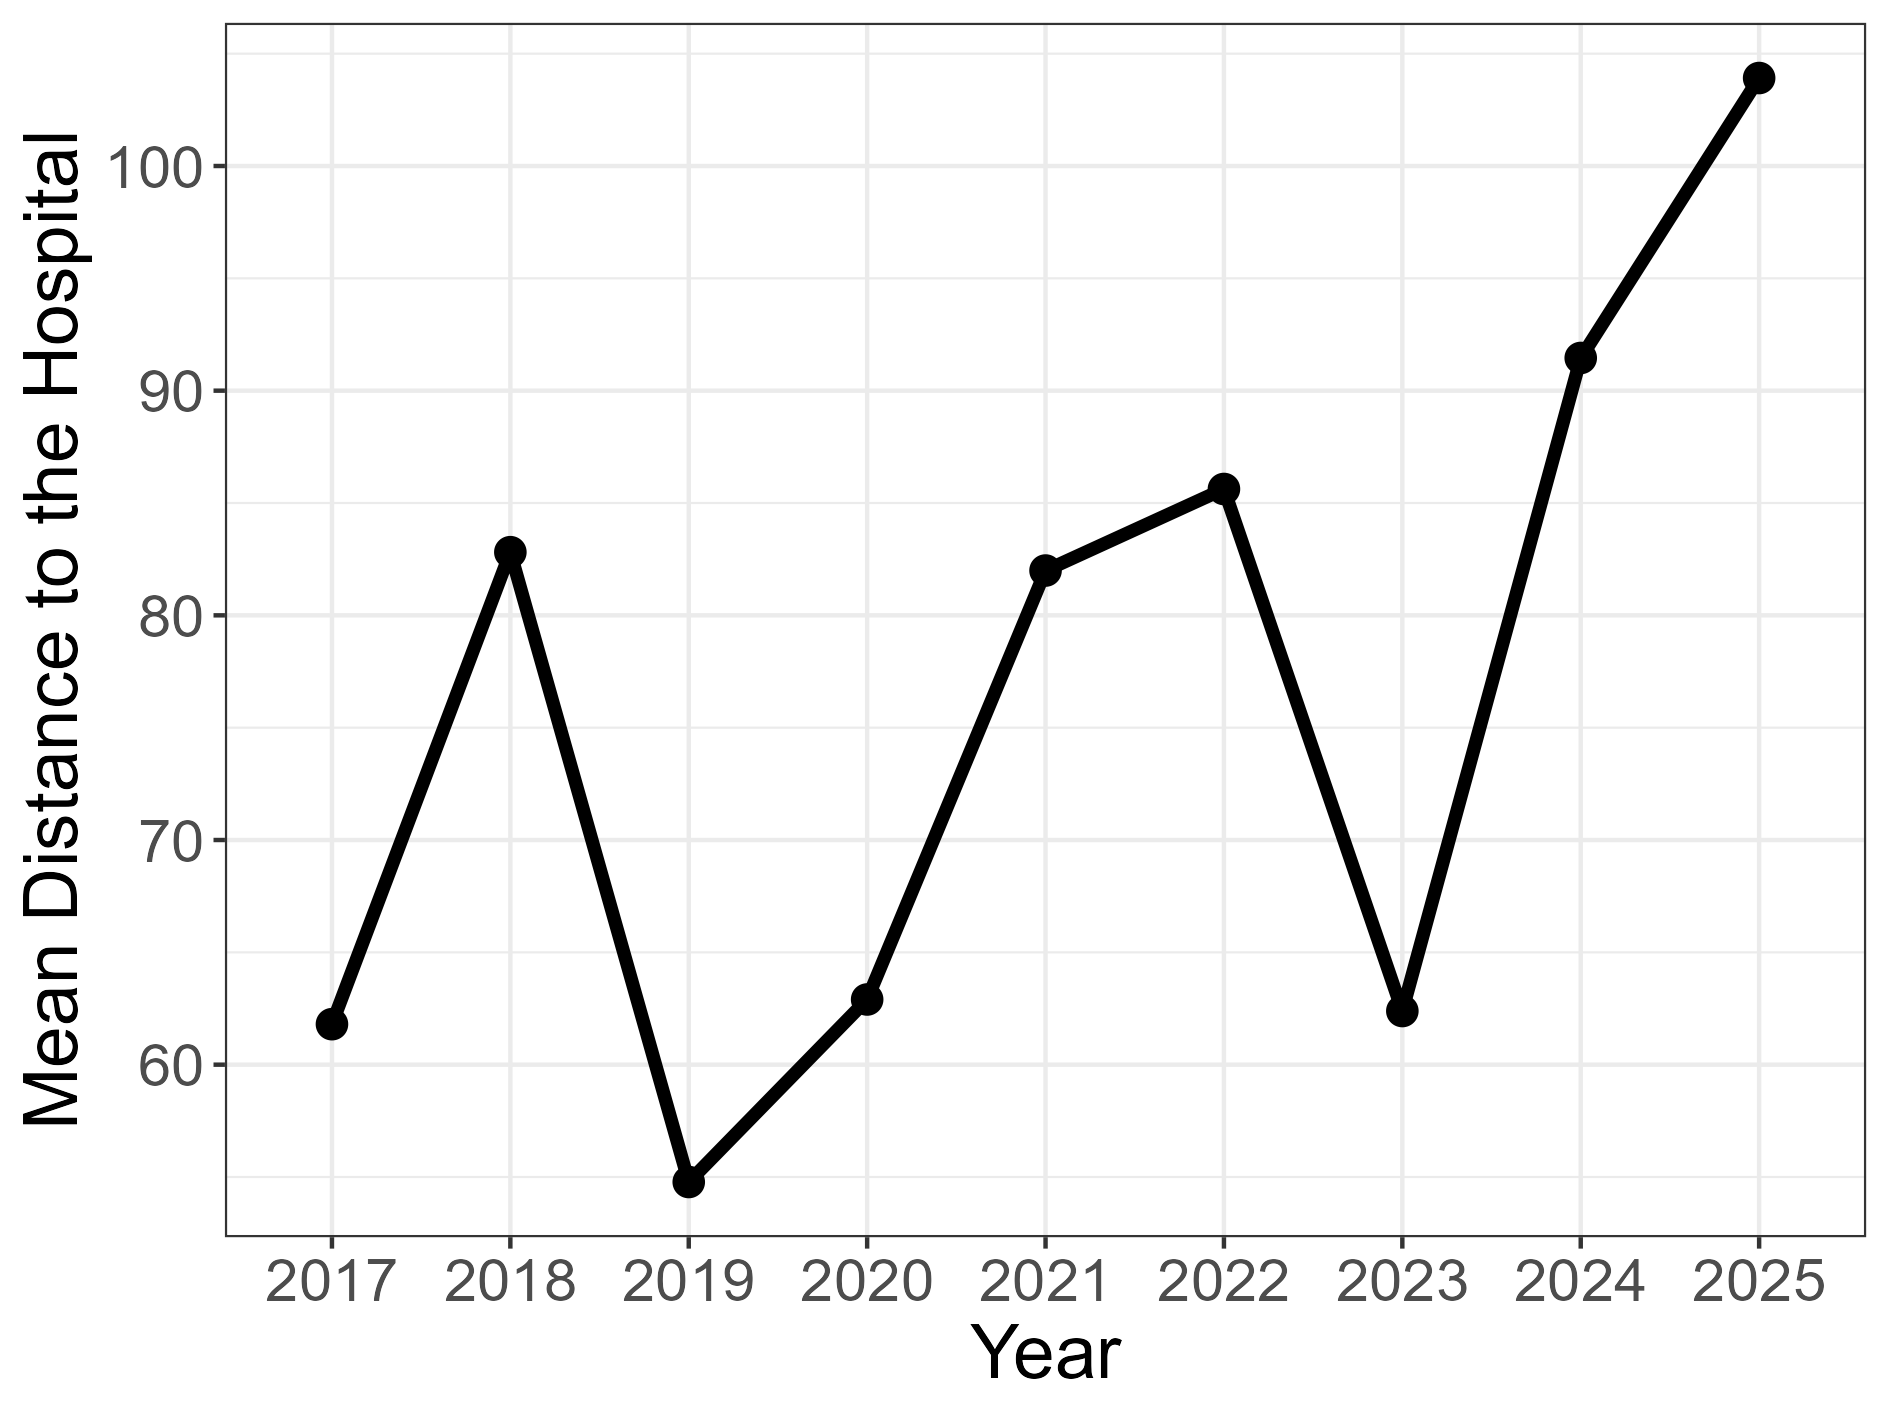
\includegraphics[width=0.75\textwidth]{nutri_paren_id_dist.png}
    \caption{Mean travel distance (km) between the patient's residential postal code centroid and the municipality of the admitting hospital, among identified CIF patients, by year, Brazil, 2017--2025.}
    \label{fig:distancia}
\end{figure}

\begin{figure}[H]
    \centering
    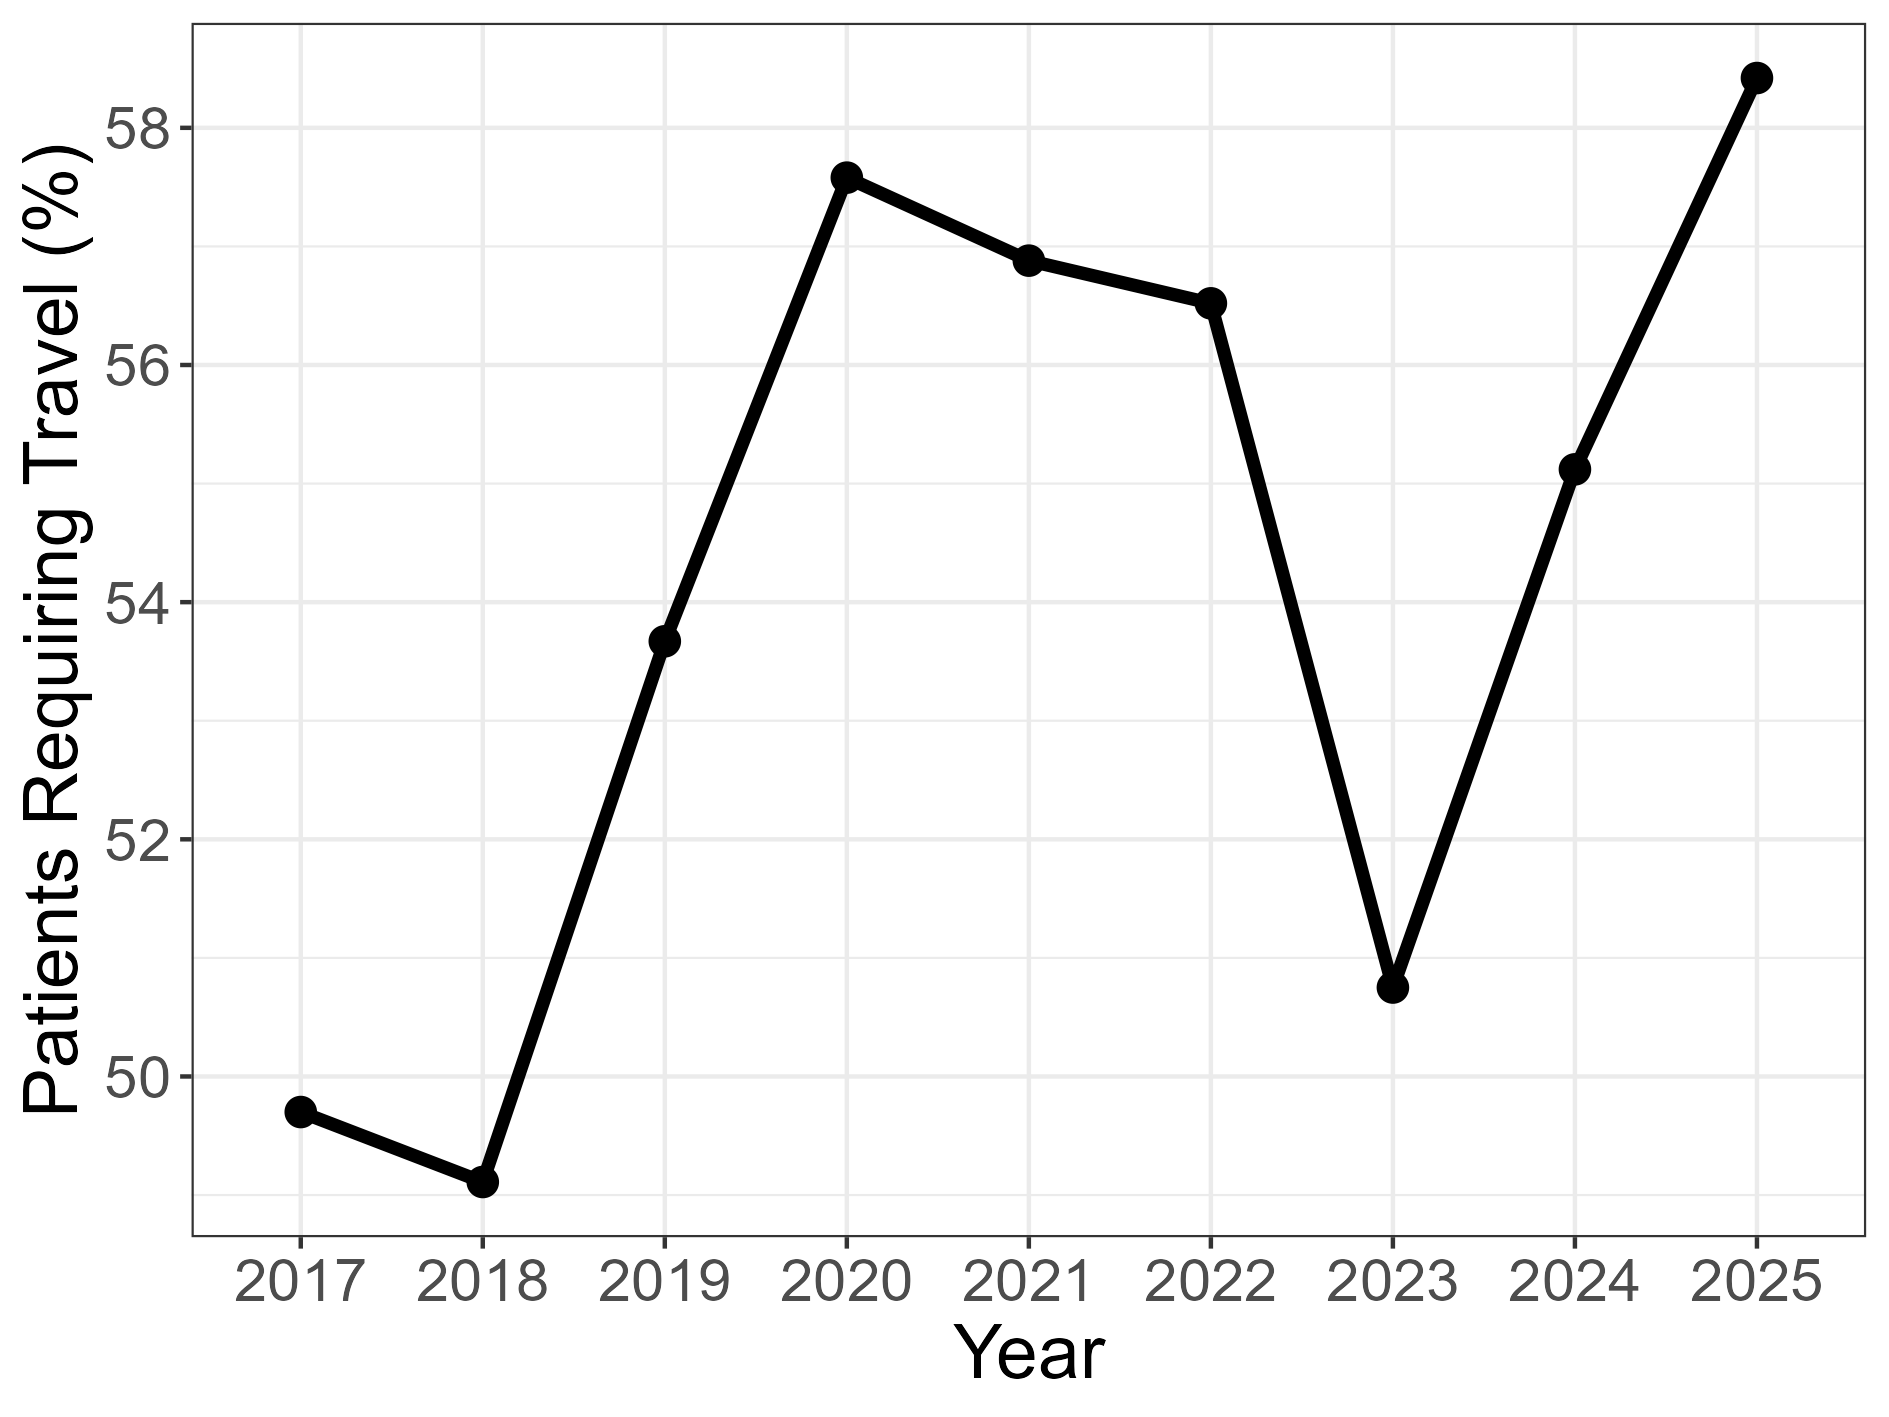
\includegraphics[width=0.75\textwidth]{nutri_paren_id_desloc.png}
    \caption{Proportion of identified CIF patients required to travel outside their municipality of residence to access parenteral nutrition, by year, Brazil, 2017--2025.}
    \label{fig:deslocamento}
\end{figure}

The combination of high geographic displacement, low prevalence estimates relative to international benchmarks, and a mortality rate that exceeds what is achievable with adequate treatment collectively point toward a scenario in which a meaningful proportion of CIF cases in Brazil are not being captured by administrative data, either because they lack access to specialised care altogether, or because they are treated in institutions that record PN procedures under non-specific codes. This possibility is directly examined in the following section.

\subsection*{Complementary Analysis: Evidence of Systematic Underreporting in CIF-Specific Procedure Codes}

To assess the extent to which the PN-based prevalence estimates reflect genuine access to CIF care rather than the full scope of the condition, we examined hospital admissions recorded under the new intestinal failure rehabilitation code at the hospital level (03.01.16.002-3), introduced by the Brazilian Ministry of Health in August 2024 through Portaria GM/MS N\textordmasculine~5.051/2024. If the new code were being systematically adopted across the hospitals that manage paediatric CIF in Brazil, one would expect the number of cases recorded under this code to approach the annual case counts derived from the PN-based strategy. The results indicate that this is far from the case.

Between August 2024 and December 2025, only 86 hospital admissions were recorded under the new code in the entire SIH-SUS, corresponding to 22 unique patients after deduplication. Among these 22 patients, 13 (59.1\%) were female, none were classified as non-white in the administrative record, all were aged 12 years or younger, 9 had admissions lasting fewer than 30 days, and 8 had admissions lasting more than 60 days. The most frequently registered diagnoses were unspecified intestinal malabsorption (K909, $n = 36$), other forms of intestinal malabsorption (K908, $n = 20$), other forms of intestinal obstruction (K566, $n = 16$), post-surgical malabsorption (K912, $n = 8$), and malabsorption due to unspecified intolerance (K904, $n = 6$).

Most strikingly, all 86 admissions were recorded by only two hospitals in the entire country --- the Hospital de Cl\'{i}nicas of Porto Alegre (56 admissions) and the Hospital das Cl\'{i}nicas of S\~{a}o Paulo (30 admissions) --- and the overwhelming majority of patients resided in municipalities located in the state of Rio Grande do Sul (Table~\ref{tab:municipios}). This extreme concentration in two institutions strongly suggests that the low case count reflects not the true national burden of paediatric CIF but rather a near-complete failure of the new code to diffuse into routine clinical coding practice outside a small number of specialised centres. Whether this reflects a lack of awareness of the new coding requirements, insufficient training of coding staff, or the institutional inertia that typically accompanies the introduction of new procedure codes in large administrative systems remains uncertain. What the data make clear, however, is that the 22 cases identified through the new code represent a small fraction of the approximately 80 to 148 annual cases identified through the PN-based strategy in the same period, a discrepancy of an order of magnitude that cannot be attributed to differences in case definition alone.

\begin{table}[ht]
\centering
\caption{Municipalities of residence of patients identified through the new intestinal failure rehabilitation procedure code (03.01.16.002-3), Brazil, August 2024--December 2025.}
\label{tab:municipios}
\begin{tabular}{lc}
\toprule
Municipality of residence & No.\ of procedures \\
\midrule
Rolante/RS & 4 \\
Arroio do Tigre/RS & 3 \\
Mandaguari/PR & 1 \\
Alvorada/RS & 1 \\
Porto Alegre/RS & 1 \\
Rio Pardo/RS & 1 \\
Viam\~{a}o/RS & 1 \\
\bottomrule
\end{tabular}
\end{table}

Taken together, these findings provide direct empirical support for the interpretation advanced throughout this results section: that the PN-based prevalence estimates reported here capture only the portion of the paediatric CIF population that successfully accessed prolonged parenteral nutrition within the SUS and whose care was recorded under a relevant procedure code. The low uptake of the CIF-specific code introduced in 2024, even in the context of an explicit national policy mandate, illustrates the broader challenge of generating reliable epidemiological data on rare conditions within large, heterogeneous administrative health systems, and underscores the likelihood that the true prevalence of paediatric CIF in Brazil is meaningfully higher than the figures reported here.

\section{Discussion}\label{sec4}

[Apoio Ivan]

We describe a ... (...) This is comparable to reports from other

\cite{khokhar2025global} - melhor artigo para introdução e depois discussão com relação a estimativa pela nutrição.

These studies reported ((...). The differences in the estimates

Additionally,

\cite{leite2025multicenter} - Na discussão ausência de dados gerais para o Brasil. Estudo relevante recente que analisou 207 pacientes em 3 centros das regiões Centro Sul (SP e PA) sequer cita dados gerais para o Brasil. O que o artigo aborda em relação ao panorama brasileiro é que o cenário de reabilitação intestinal no país é altamente desafiador
. Os autores destacam que, como o Brasil é um país de renda média, o tratamento esbarra em problemas como:
Recursos financeiros limitados;
Acesso insuficiente aos poucos centros de referência existentes;
Falta de treinamento adequado para equipes multidisciplinares;
Atrasos no diagnóstico devido à baixa conscientização sobre a doença;
Desafios logísticos e estruturais para a implementação segura da Nutrição Parenteral Domiciliar (NPD).


Avaliar se vale linkar com heterogeneidades geográficas no Brasil e populações mais vulneráveis - \cite{pant2017epidemiology} - Black children had a disproportionately greater representation in the SBS cohort. It may be possible that this is linked to disparity in income; low socioeconomic status is a risk factor for preterm birth. / Children hospitalized with SBS have a complex disease with a
high severity of illness and are especially vulnerable


\section*{Strengths and limitations}

To our knowledge, this is the first study to estimate the national prevalence of pediatric Chronic Intestinal Failure in Brazil using population-based administrative hospital data. A major strength of this analysis is the use of detailed SIH-SUS/AIH records over a nine-year period, which allowed us to identify prolonged parenteral nutrition exposure at the admission level and to construct a longitudinal proxy for CIF in the absence of a specific ICD-10 diagnosis code. The study also implemented a deterministic record-linkage strategy to reduce double counting of patients across multiple admissions, an important methodological step given that SIH-SUS records are structured at the hospitalization rather than patient level. In addition, by combining prevalence estimation with clinical, demographic, mortality, and geographic analyses, the study provides not only a national estimate of disease burden but also evidence on access barriers, regional inequalities, and patterns of healthcare utilization. The complementary analysis using the intestinal-failure-specific procedure code introduced in 2024 further strengthens the interpretation that official coding remains incomplete and that CIF is likely underreported in routine administrative systems.

This study also has several limitations. First, case identification relied on prolonged parenteral nutrition as an operational proxy for CIF. Although this approach is clinically grounded and consistent with the chronicity criterion used in the literature, it may misclassify some patients: children receiving long-term PN for reasons other than CIF may have been included, while patients with CIF who did not access prolonged hospital-based PN, received home PN, were treated in the private sector, or had their procedures recorded under non-specific codes may have been missed. Second, SIH-SUS does not include a persistent patient identifier, requiring deterministic linkage based on postal code, sex, and date of birth. This strategy reduces duplicate counting but may still generate linkage error, particularly in cases of missing or inaccurate administrative fields. Admissions with missing postal code information also had to be excluded, which may have introduced selection bias. Third, because SIH-SUS captures only hospitalizations reimbursed by the public health system, national counts were adjusted using a scaling factor based on the overall public-private distribution of hospital admissions. This assumes that CIF care follows the same distribution as hospital admissions in general and that this relationship remained stable over time, assumptions that cannot be directly verified with available data. Fourth, the study is based on billing records rather than clinical registries; therefore, information on underlying anatomy, residual bowel length, enteral autonomy, home parenteral nutrition, long-term survival, quality of life, and outpatient follow-up was unavailable.

Nevertheless, these limitations are more likely to lead to underestimation than overestimation of the true burden of pediatric CIF in Brazil. The low prevalence estimates observed in this study, the incomplete recovery after the COVID-19 pandemic, the concentration of care in a small number of hospitals, and the minimal uptake of the new CIF-specific procedure code all point to substantial underdiagnosis, underreporting, and unequal access to specialized treatment. Therefore, the estimates presented here should be interpreted as a lower bound of the national burden and as a starting point for the development of prospective registries, standardized coding practices, and coordinated referral networks for children with CIF in Brazil.


\section{Conclusions}\label{sec5}

[Ivan e Pedro avaliar e amarrar]

While acknowledging the limitations of administrative records, this study provides the first population-based estimate of pediatric Chronic Intestinal Failure (CIF) prevalence in Brazil. Our findings suggest a profound epidemiological underestimation compared to high-income settings, reflecting structural barriers to timely diagnosis and prolonged nutritional therapy rather than biological rarity. Furthermore, the observed geographic disparities illustrate how the lack of specialized infrastructure in most regions imposes severe logistical burdens on families, contributing to unfavorable clinical outcomes and hidden mortality.

For healthcare providers and policymakers, these results suggest key areas for strengthening the current care pathway. Enhancing support within the Unified Health System (SUS) could involve establishing multidisciplinary teams nationwide to improve regional care capacit. (...)


\section*{Acknowledgements}

This work was supported by Pensi Institute and Jose Luiz Setubal Fundation. The authors bear full responsibility for the content of this study.

\section*{Author Contributions}

All authors wrote, reviewed and approved the final version of the manuscript.

\section*{Conflict of interest/Competing interests}
The authors have no conflict of interest to declare.

\section*{Ethics approval and consent to participate}
Not applicable due to the nature of the study being work public data.

\section*{Data availability}
The datasets and codes generated during the current study are available from the corresponding author on reasonable
request.

\newpage
\begin{appendices}

\section{First appendix}\label{secA1}

[Final]

\end{appendices}


\newpage
\bibliographystyle{plainnat}
\bibliography{biblio}

\end{document}
